\documentclass[a4paper,11pt,UKenglish,twoside,openright]{report}\usepackage[]{graphicx}\usepackage[]{color}
% maxwidth is the original width if it is less than linewidth
% otherwise use linewidth (to make sure the graphics do not exceed the margin)
\makeatletter
\def\maxwidth{ %
  \ifdim\Gin@nat@width>\linewidth
    \linewidth
  \else
    \Gin@nat@width
  \fi
}
\makeatother

\usepackage{Sweavel}



\usepackage{uiothesis}

\title{Identifying School Climate Variables Associated with Financial Literacy Outcomes in PISA 2018 Data}
\subtitle{A Multilevel Structural Equation Modelling Approach}
\author{Tony C. A. Tan}

\begin{document}

% Input faculty etc info
\duoforside[
    fac={Faculty of Educational Sciences},
    dept={Centre for Educational Measurement},
    program={Science (Assessment, Measurement and Evaluation)},
    date={Spring 2021},
%  printer={X-press printing house},
    short
]

% Change page numbering to roman
\pagenumbering{roman}

% Create an acknowledgement page
\thispagestyle{empty}

% This is where I generated the Chinese characters
%//ref http://www.akuziti.com/mb/
% I used font 24.Huawen Xingkai and 100 pixel
\vspace*{\fill}
\begin{figure*}[h]
    
\includegraphics[width=\textwidth]{./Figures/To-parents.png}
\end{figure*}
\begin{flushright}
To my parents
\end{flushright}
\vspace*{\fill}
%\newpage
\clearpage
\thispagestyle{empty}

\vspace*{3cm}

\begin{quote}
    \calligra\huge      % Changes the font to caligraphy and huge size.
\hyphenchar\font=-1     % Stops LaTeX from splitting/hyphenating words
Study hard what interests you the most in the most undisciplined, irreverent and original manner possible.
\end{quote}

\begin{figure*}[h]
    \flushright
    
\includegraphics[width=0.50\textwidth]{./Figures/Feynman-Signature.jpg}
\end{figure*}
\vspace*{-1cm}

%\begin{flushright}
%--- Richard P. Feynman
%\end{flushright}

\setcounter{page}{0}
% End of acknowledgement page

% Put Table of Content here
\tableofcontents

% Put a List of Tables here
\listoftables

% Put a List of Figures here
\listoffigures



% APA7 Rule 2.21 Line Spacing
%\onehalfspacing
\doublespacing

% Acknowledgement

\chapter*{Acknowledgement}
\label{Ac}

Thank-you goes to

% Popular Abstract

\chapter*{Popular Abstract}
\label{Ab.0}

Preparing youth for life-long success with numeracy, literacy and science capability has been the foundation for all schooling. The post-global financial crises and post-COVID era, in addition, imposes increasing demand on financial literacy for school leavers. Since 2012, OECD has been a pioneer in measuring 15-year-olds' financial literacy through its triennial Programme for International Student Assessment (PISA) cycles. Subsequent analyses using PISA data, however, reported paradoxical results that more classroom interventions tend to be associated with either no differences or even lower scores in students' financial literacy measures. It is in educators' interest therefore to carefully examine the relationship between school climate variables, including the academic, safety, community and institutional envrionment aspects of students' lives, and their financial literacy outcomes.

[Project summary]

The motivation for this project originates from my confusion over the current stock of literature, which states that school efforts do not matter, even harmful, in bringing about students' financial literacy while homes are better suited for this purpose. This claim is worrisome because if school are committing something wrong, school leaders and policy makers genuently want to know what, which and where so that harmful pedagogies can be reverted into good practices. Alternatively, it could also be the measurement instrument researchers employed so far that led to such underwhelming results. A closer examination of how school effectiveness is measured would also promote research practice and the resultant policy advice.

Using 2018 PISA financial literacy data, including all 20 participating countries, I was able to examine how school climate variables, namely ACADEMIC, SAFETY, COMMUNITY and INSTITUTIONAL ENVIRONMENT each explained the total variation in students' financial literacy outcomes. Using a multilevel SEM with students' finance-related affective variables as mediators, my random intercept model shows that schools' academic practices do matter in advancing students' financial literacy outcomes but only through affective pathways. Cognitive pathways, however, were shown to correlate negatively with financial literacy scores. Since schools' congnitive and affective pathways are similar in size but opposite in signs, combining the two into total effects would have inadvertently resulted in the nonfindings as reported by prior literature. In addition to this methodological insight, countries that overly focused on accountability through standard testing, tracking and measuring students' financial skills (e.g., the USA) fell prey to this cognitive trap while countries that placed more emphases on cultivating students' affective affinity such as confidence in, and familiarity with, financial matters (e.g., Finland) delivered impressive education outcome in financial literacy.

% Abstract

\chapter*{Abstract}
\label{Ab.1}

Repeated economic crises in recent memory have exposed the harsh consequences of financial \emph{illiteracy} shared by high proportions of the general population. Policy makers experienced little resistance when identifying youth as the most effective group for bringing about improvement in citizens' ability to engage with economic and financial matters, but opinions quickly diverge over the optimal approaches for achieving such targeted outcome. Existing literature frequently reports the importance of family environment in cultivating students' financial literacy through the process of ``financial socialisation'' -- [definition goes here] (reference). Such practice, however, encounters interrogation by educators over equity concerns should families remain the main arena for financial literacy development. Schools play vital roles in alleviating inequality in accessing education and training in general but scarce research so far has been devoted into identifying the specific classroom factors that are most effective in advancing students' financial literacy outcomes. The current study therefore attempts to contribute to this enquiry by investigating the relationship between school climate variables and students' financial literacy achievement with an aim of stimulating policy debate about the levers and instruments available to education interventionists for the purpose of improving young people's financial literacy and preparedness as they step into an increasingly uncertain world. Using the 2018 PISA dataset, this paper employs a three-level hierarchical model to conduct cross-country comparisons to highlight school climate variables that are most strongly associated with high financial literacy outcomes.

% End of front matter. None of the pages so far counts towards the page limit.
\clearpage
\thispagestyle{empty}

% Restart page number. Page count starts here.
\pagenumbering{arabic}
\setcounter{page}{0} % Do not swap these two command. Need new chapter to be "Open right".

% Chapter 1 Introduction

\chapter{Introduction}
\label{chp:1}

%\epigraph{If you think education is expensive, try ignorance}{Derek Bok}

%//mark Broad motivation

Repeated economic crises in recent memory have exposed the harsh consequences of financial \emph{illiteracy} shared by high proportions of the general population. Low financil literacy was directly linked with negative credit behaviours such as high amount of credit card debt \parencite{meier:2010}, high costs of borrowing, poor mortgage choices and subsequent delinquency and home foreclosure \parencite{hastings:2013}. Poor financial decisions made early in life can have profound long-term economic and societal impacts \parencite{montoya:2013} such as forgoing medical care \parencite{lusardi:2015}, mental health crises \parencite{stone:2018} and geriatric poverty resultant from insufficient retirement provision \parencite{lusardi:2007, lusardi:2008}.

Even more concerning is the pervasive global distribution of financial illiteracy. Deficiencies in financial capability had been observed not only in emerging economies \parencite{karakurumozdemir:2019} such as Colombia \parencite{caoalvira:2020}, Mexico \parencite{arceogomez:2017, bohm:2021}, India \parencite{agarwal:2015, kiliyanni:2016, utkarsh:2020}, Indonesia \parencite{cole:2009, khoirunnisaa:2020}, Turkey \parencite{akbenselcuk:2014}, and Eastern European countries \parencite{belas:2016, opletalova:2015, reiter:2020} but also in advanced economies such as Australia \parencite{ali:2014, taylor:2013, thomson:2017}, Canada \parencite{boisclair:2017}, Germany \parencite{bucherkoenen:2017, erner:2016}, Austria \parencite{silgoner:2015}, the UK \parencite{barnard:2021} and the USA \parencite{breitbach:2016, gale:2012, huston:2012, lusardi:2010}. International comparisons also reported low financial literacy in many Asian \parencite{yoshino:2015} and OECD countries \parencite{cupak:2018a, lusardi:2015a}, particularly amongst the young \parencite{debeckker:2019}, females, lower educated \parencite{klapper:2019} and somewhat surprising, inhabitants of countries with more generous social security systems \parencite{jappelli:2010}.

One major reason behind the escalating interests in citizens' financial literacy can be attributed to the policy adjutment taking place in the past two decades. The neo-liberal ideology of reducing government involvement in the economy had crowded out societal care such as pension, health and education from the collective via the state to the individuals \parencite{gilbert:2002}. In a post-financialisation world \parencite{krippner:2005}, the primary goal of political economy has shifted from the redistribution of wealth to the \emph{incorporation} of individuals within the mainstream financial architecture \parencite{regan:2003}. The succession of the asset-based welfare system to the income-based model \parencite{finlayson:2009}, however, was by no means unique to the Anglosphere. The Hartz reforms of 2003/04, according to \textcite{seeleibkaiser:2016}, had significantly altered Germany's post-war social welfare arrangement, leading \textcite{ferragina:2015} to re-classify Germany into a liberal welfare state comparable to the United Kingdom. Although a detailed account of the history, politics and moral philosophy of social welfare reforms is beyond the scope of this project, it suffices to highlight financial litearcy as a social necessity to avoid harm and hardship, especially to today's young.

Research efforts aiming at advancing youth's financial literacy over the years evolved into two strands: on the design and evaluation of school financial education programs, and on the influence of home environment through the process of financial socialisation---the intentional or involuntary transmission of financial concepts which are required to functioning successfully in society \parencite{bowen:2002}. A recent meta-analysis conducted by \textcite{kaiser:2020} found that while school financial education programs had sizeable impacts on \emph{financial knowledge} ($+0.33\ SD$) similar to education interventions in other domains, their effect on students' \emph{financial behaviour} is quite small ($+0.07\ SD$). This conclusion added to a list of weak or non-findings regarding the long-term behavioural effect brought about by school financial education programs. \textcite{brown:2016}, for instance, reported mixed outcome in students' long-term financial well-being depending on the programs received; whereas \textcite{cole:2016} observed that traditional personal finance courses lacked any explanatory power in accounting for graduates' financial outcome once the additional mathematics training in which finance topics were packaged has been controlled for. Despite careful controls and thoughtful study designs, correlating classroom interventions and young people's financial literacy outcomes has repeatedly yielded paradoxical results of non-significant or even negative relationship; any positive findings remain small in magnitudes and/or are sensitive to robust analyses.

Optimism, fortunately, runs higher at the financial socialisation camp. Building on the acknowledgement that families serve as information filters from the outside world \parencite{danes:2007} as well as the foundation for youth's continued financial concept formation, \textcite{gudmunson:2011} put forward a family financial socialisation theory to accommodate both the \emph{process} and the \emph{outcome} for variations in young people's financial capabilities. Using structural equation modelling, \textcite{jorgensen:2010} was able to show that perceived parental influence had a direct and moderately significant influence on financial attitude, did \emph{not} have an effect on \emph{financial knowledge}, and had an indirect and moderately significant influence on financial behaviour, mediated through financial attitude. This attitude(A)--behaviour(B)
--cognition(C) conceptualisation of financial literacy \parencite{potrich:2015} continues to influence subsequent research effort. More recently, \textcite{morenoherrero:2018a} continued this line of enquiry by applying multilevel regression analyses to 2015 PISA data and reported that students' financial literacy was associated mainly with understanding the value of saving and discussing money matters with parents. In addition, exposure and use of financial products, in particular holding a bank account, improved students' financial knowledge as well.

One chief concern for every research project is the quality of its data source. Amongst competing inventories, PISA stands out as a comprehensive and reliable source of data for measuring 15-year-olds' financial literacy outcomes thanks to OECD's careful sampling procedure and attention to construct validity of measurement. Four technical features of PISA are crucial for the architecture of this study. First, following statistical theory, PISA designers acknowledged the hierarchical nature of education research data such that students are nested in schools, and schools are further nested in countries. Second, one student weight is assigned to each observation in order to account for the fact that not all schools in a country are equally likely to be sampled by the PISA organiser; and given a particular school that has been chosen, not every student in this school is equally likely to be asked to participate in the test \parencite{rust:2014}. A third complication arises from the ``planned missingness'' in students' responses because each participant is only given a small number of questions relative to the entire test bank in order to ensure their responses are not undermined by tiredness \parencite{vondavier:2014}, leading to the outcome variables being represented by ten plausible values. Fourthly, PISA consulted and synthesised multiple schools of thoughts \parencite{PISAframework} before constructing financial literacy as \blockquote{the knowledge and understanding of financial concepts and risks, and the skills, motivation and confidence to apply such knowledge and understanding in order to make effective decisions across a range of financial contexts, to improve the financial well-being of individuals and society, and to enable participation in economic life. (p. 128)} As a result, 2018 PISA data set \parencite{FLdata} provides not only variables measuring \emph{cognitive} outcomes but also \emph{affective} factors such as familiarity with concepts of finance and confidence about financial matters, enabling a nuanced study design involving decomposing the total effect of financial literacy development into its ``brain'' (cognitive) and ``heart'' (affective) pathways.



%//mark Definition of key terms

%//mark My topic(s)

%//mark Zoom out: Why is this topic important?


\section{Profiles of Successful Learners}

\subsection{Social, Economic and Cultural Status}

\subsection{Immigration History}

\subsection{Sex Differences}


Not all high school graduates continue into tertiary education and only a portion of the latter group receive further training in finance-related areas, senior years in secondary education present an ideal interval for introducing financial literacy intervention as it captures the widest participant base \parencite{walstad:2016}.





Financial literacy can be seen as an investment in human capital \parencite{lusardi:2014}. Today's young people are growing up in a society in which the financial landscape is complex and the financial responsibilities of citizens are substantial.






\section{Research Questions}\label{sec:rq}

% APA7 Rule 6.50 Lettered Lists and 6.51 Numbered Lists
The current study wishes to take advantage of the latest wave of 2018 PISA results and investigate the covariation financial literacy outcomes share with the following four aspects of young people's daily lives, inspired by school climate literature. More specifically, this project aims to answer these two research questions:
\begin{enumerate}
    \item[RQ1.] To what extent can the variation in students' financial literacy outcomes be accounted for by each of the school climate variables?
    \item[RQ2.] How does the school environment impact on individual learners' financial literacy acquisition process?
\end{enumerate}

% Chapter 2 Theoretical framework

\chapter{Conceptual Framework}
\label{chp:2}

%//mark In-depth definitions of ``financial literacy''

%//mark Define every term my readers need in order to understand my research question

%//mark Survey not only PISA but also alternative definitions, even critiques of such definitions

%//mark Any practices that are common in maths/literature but uncommon in financial literacy? Meaning? Implies?

This chapter provides in-depth explanations of the two concepts underpinning this research project: \poscite{wang:2016} school climate framework and PISA 2018's approach to quantifying students' financial literacy. In particular, it reviews existing literature on the impact of school intervention (the academic aspect of school climate) and parental involvement (the community aspect) on youth's financial literacy development in \cref{sec:sc} and how PISA 2018 measured students' financial knowledge, confidence as well as their application of which into financial decision-making in \cref{sec:flit}.

\section{School Climate}\label{sec:sc}

A positive school climate is easier to recognise but difficult to define, even to the present day \parencite{PISAvol3}. When organising school attributes into frameworks, early studies loosely clustered themselves into two camps along the concrete--abstract spectrum. When researching on students' behavioural problems and emotional distress, for example, \textcite{kuperminc:1997} recognised the insufficiency of using observable characteristics of a school as the metric for its managerial success but adopted a utilisation and perception approach based on social-ecological and developmental theories. Such emphasis on school users' \emph{perception} continued into \textcite{esposito:1999}'s study of students' social disadvantages on their academic outcomes, with EFA results suggesting a five-factor model including student academic orientation, parent-school relationships, security, administration and teacher-student relationships. \textcite{freiberg:1999}, on the other hand, took a more idealised view of school climate as ``the heart and soul of a school''---the very ``essence of a school that leads a child, a teacher, an administrator, a staff member to love the school and to look forward to being there each school day'' (p. 11). However broad or narrow the definition, both ends of the spectrum signalled that the ultimate utility of any school climate framework should facilitate our understanding of student development.

With this goal in mind, \textcite{wang:2016} surveyed six theories for the purpose of building a multidimensional school climate framework. Since schooling is an interaction between individuals and every envrionment immersing them (the bio-ecological theory), students inevitably develop protective and/or maladaptive behaviours (risk and resiliene perspective) in addition to all existing bond they formed with parents (attachment theory). Thanks to students' ever growing capabilities, schools may then encourage learners to connect, invest, participate and believe in their immediate environment (social control theory), by bridging their motivation towards success criteria (social cognitive theory) and by removing barriers (stage-environmental fit theory) to growth. These theories jointly guided a literature review and coding exercise that led to a four-domain, 13-dimension structure of school climate framework \parencite[see Figure 1,][p. 318]{wang:2016}. This research project approached \poscite{wang:2016} ontology from the domain-level and referred the \emph{academic} climate as the overall quantity and quality of the teaching-learning activities; \emph{community} as the engagement and interpersonal ties schools maintain with stakeholders particularly parents; \emph{safety} as the degree of physical and emotional security afforded by schools; and \emph{institutional environment} as the organisational and structural features of schools in particular their educational resource availability. All four branches of the school climate framework serve as platforms upon which students' financial literacy can be constructed.

\subsection{School Financial Education Programs}

Amongst the many redress schemes aimed at promoting citizens' financial capability, the return on investment is the highest when intervention is applied as direct classroom interventions to the young. \textcite{lusardi:2014} have shown that providing financial knowledge to high schoolers before they enter the labour market increases their well-being by approximately 82\% of their initial wealth, while the rate of return is around 56\% for college graduates.

\subsection{Parental Influence and Financial Socialisation}

Although financial capability is an important integral of adulthood, the process of acquiring the financial knowledge and skills begins in early childhood. Parents provide a context in which children learn what money is, for instance, and how it is used and saved \parencite{birbili:2015}. Whether intentionally or informally, financial intuition is passed around the household through frequent interactions, conversations, and lessons. Consequently, the financial knowledge and skills acquired while growing up at home form the foundation for the financial attitudes and behaviours carried into adulthood \parencite{serido:2016}. Using panel data set from the Dutch DNB Household Survey between 2000 and 2012, \textcite{bucciol:2014} reported that parental teaching about savings increased the likelihood of adult saving by 16\% and the saving amount by approximately 30\%. Similar intergenerational effect was observed from longitudinal studies in the US, linking adolescents' observation of parents' responsible financial behaviour to their own good decisions and actions later in life \parencite{tang:2017}.

\subsection{School Safety}


While it is well established that adverse safety experience at school reduces academic attainment \parencite{kutsyuruba:2015}, the specific evidence linking bullying to financial literacy underperformance is scarce in comparison.

\subsection{School Resources}

\section{Financial Literacy}\label{sec:flit}

In its official publication \textit{PISA 2018 Assessment and Analytical Framework} \parencite{PISAframework}, the OECD provided an explicit definition of ``financial literacy'' as
\vspace{-1em} % Eliminate the ugly spacing
    \blockquote{the knowledge and understanding of financial concepts and risks, and the skills, motivation and confidence to apply such knowledge and understanding in order to make effective decisions across a range of financial contexts, to improve the financial well-being of individuals and society, and to enable participation in economic life (p. 128)}
\vspace{-1em} % Eliminate the ugly spacing
with emphases on both the thinking and behaviour that characterise such construct and the purposes for developing this particular literacy. Of particular relavence to the current project are the knowledge, confidence and application aspects of financial literacy.

%//mark Briefly explain PISA here.

\subsection{Knowledge Aspect of Financial Literacy}

Since poor financial behaviours have been associated with a lack of financial knowledge \parencite{hastings:2013, lusardi:2014}, the ultimate goal of financial literacy interventions is to ensure students receive the information and support they need to make responsible and appropriate financial decisions confidently, both in their school years and in adult lives \parencite{PISAvol4}. In order to ascertain candidates' current understanding of finance-related topics, \textsf{FL164} of the financial literacy questionnaire presented 18 terminologies such as exchange rate, budget, and income tax and asked students to rate their familiarity with each term using a three-point scale: ``Never heard of it'', ``Heard of it, but I don't recall the meaning'' and ``Learnt about it, and I know what it means''. Sum scores of \textsf{FL164} were used to construct ``familiarity with concepts of finance'' variable (\texttt{FCFMLRTY}, Chapter 16 of \textit{PISA 2018 Technical Report}, \textcite{PISAtech}, p. 23), which is expected to share a positive correlation with students' financial literacy performance.

\subsection{Confidence Aspect of Financial Literacy}

The positive association between students' confidence and their academic attainment has also been well documented. By sythesising one decade of large-scale international assessment data, \textcite{lee:2018} found self-beliefs (labelled ``self-efficacy'' in PISA and ``confidence'' in TIMSS) to be the strongest non-cognitive predictor for students' mathematics achievement. Similar relationships had also been observed in the realm of financial literacy such as \poscite{arellano:2014} study using the Spanish portion of the PISA 2012 financial literacy data, and \poscite{borgesramalho:2019} results based on the Brazilian sub-sample of the 2016 OECD/INFE International Survey of Adult Financial Literacy Competencies. PISA 2018 therefore included a set of questions in \textsf{FL162} asking students about their confidence over six financial activities such as making money transfers, understanding bank statements, and plan their spendings using a four-point Likert scale ranging from ``Not at all confident'', ``Not very confident'', ``Confident'' to ``Very confident''. A variable ``confidence about financial matters'' was subsequently constructed using the IRT procedure (\texttt{FLCONFIN}, \textcite{PISAtech}, p. 23) and is expected to have a positive association with financial literacy performance in the current study.

\subsection{Application Aspect of Financial Literacy}

% Table generated by Excel2LaTeX from sheet 'Sheet1'
\ptable{tab:FLIT}{Structure of PISA 2018 Financial Literacy Construct}{
      \begin{tabular}{c @{\hskip 2cm} l @{\hskip 2cm} c}
      \toprule
            &       & Distribution of \\
            Domain$\, ^\text{a}$ & \multicolumn{1}{c}{Content areas} & score points (\%) \\
      \midrule
      Content & Money and transactions & 30--40 \\
            & Planning and managing finances & 25--35 \\
            & Risk and reward & 15--25 \\
            & Financial landscape & 10--20 \\
            &       &  \\
      Process & Identify financial information & 15--25 \\
            & Analyse information in a financial context & 15--25 \\
            & Evaluate financial issues & 25--35 \\
            & Applying financial knowledge and understanding & 25--35 \\
            &       &  \\
      Contexts & Education and work & 10--20 \\
            & Home and family & 30--40 \\
            & Individual & 35--45 \\
            & Societal & 5--15 \\
      \bottomrule
      \end{tabular}
}{This table synthesised Table 5.1 to 5.3 of \textit{PISA 2018 Assessment and Analytical Framework} \parencite[][p. 155]{PISAframework}. The PISA organiser used the term ``score points'' instead of ``items'' because, by questionnaire design, partial credits can be awarded for some questions.\\
$^\text{a}$ \emph{Content} comprises the areas of knowledge and understanding that are essential in the area of literay in question; \emph{processes} describes the mental strategies or approaches that are called upon to negotiate the material; and \emph{contexts} refers to the situations in which the knowledge, skills and understandings of the domain are applied, ranging from the personal to the global. \parencite[][pp. 130--131]{PISAframework}}{3}

Although financial knowledge and confidence forms the very foundation upon which financial capability can be developed, it is individuals' willingness and ability to \emph{apply} their understanding through financial decision-making that counts as the ultimate outcome of their financial literacy \parencite{huston:2010}. The financial literacy application problems were drawn from 43 questions distributed across 24 booklets. The actual test bank remained confidential due to reusability consideration, but the OECD was able to provide examples that were comparable in style and difficulty in the \textit{Analytical Framework} \parencite[][pp. 133--148]{PISAframework}. These exemplar questions illustrated the domains and content areas (see summary in \cref{tab:FLIT}) PISA 2018 covered for the purpose of constructing candidates' financial literacy scores (\texttt{FLIT}). In order to succeed in the the bank statement question (Figure 5.1, \textcite{PISAframework}, p. 133), for example, students should recognise that the necessary information was presented in multiple locations of the financial document and must be identified amongst distractions then summed together. This question covered the ``money and transactions'' content area of the ``content'' domain, the ``identifying financial information'' content area of the ``process'' domain, and the ``home and family'' content area of the ``contexts'' domain.

In addition to content design, the OECD also paid particular attention to upholding financial literacy as an independt construct. Such consideration was important because one's financial capability was known to covary with both numeracy \parencite{geiger:2020, ozkale:2020a, ozkale:2020b, sole:2014} and literacy \parencite{bay:2014} skills. Empirical studies using diverse samples from the Phillipines \parencite{indefenso:2020} to Sweden \parencite{skagerlund:2018} reported correlations between numeracy and financial knowledge/literacy to be between approximately $.61$ and $.52$. In order to minimise the impact of numeracy deficiency such as low arithmetic skills \parencite{huston:2010} on students' financial literacy performance, financial formul{\ae} were never required in any problem solving and students may use the on-screen calculator at any time of the test. Furthermore, stimulus material and task statements were generally designed to be as clear, simple and brief as possible to minimise low reading ability as underperformance in application section. Both constructed- and selected-responses were used in question design and 30 out of 43 items were automatically coded by computers. Finally, ``planned missingness'' resultant from rotating booklet design was imputed into ten plausible values \parencite{vondavier:2014} centered at 500 with standard deviation of 100 \parencite{PISAframework}.

% Chapter 3 Methods

\chapter{Methods}
\label{chp:3}

\section{Sample}

This study drew its primary data source from OECD's PISA 2018 database. Responses from both student \parencite{FLdata} and school questionnaires \parencite{SCHdata} were captured and merged into a master data file using \CR's \parencite[Version 4.0.5,][]{R} \pk{intsvy} package \parencite[Version 2.5,][]{intsvy} (see \cref{R.reimport} for analysis code) including the following 20 participating countries\footnote{Australia also participated in 2018 PISA financial literacy but chose to withhold its data from public release and is therefore excluded in the current study.}: Brazil, Bulgaria, Canada, Chile, Estonia, Finland, Georgia, Indonesia, Italy, Latvia, Lithuania, the Netherlands, Peru, Poland, Portugal, Russian Federation\footnote{Moscow Region (\texttt{CNTRYID} = 982) and Tatarstan (983) have been merged into Russian Federation (643).}, Serbia, Slovak Republic, Spain, and the USA. Twelve observations without school weights were dropped, leading to a sample size of 107,162 students nested in 6,631 schools (see \cref{tab:sample} for detailed sample profile). Under PISA 2018 sampling design, all student candidates were born in the year 2002 in international grades 7 or higher (Chapter 4 of \textit{PISA 2018 Technical Report}, \textcite{PISAtech}, p. 29) and will be referred to as ``15-year-old'' in this study.

\section{Measures}
%//mark What exactly I was using to address my research question?
%//mark Sum score? Averages? One particular question?
%//mark Motivation for choosing these measures?

\subsection{School Climate Variables}

Following \poscite{wang:2016} framework, this study selected variable \texttt{FLSCHOOL} ``financial education in school lessons'' as an indicator for the academic domain of school climate; \texttt{FLFAMILY} ``parental involvement in matters of financial literacy'' (i.e., ``financial socialisation'') for the community engagement dimension, \texttt{NOBULLY} (reverse coding of \texttt{BEINGBULLIED} such that larger numbers imply safer schools) as an indicator for school safety, and lastly \texttt{EDUSHORT} ``shortage of educational material'' as an indicator of the resource availability aspect of the institutional environment of schools. All four measures were derived variables based on IRT scaling, with good scale reliabilities for most countries and constructs (see \cref{tab:cronbach} for Cronbach's alphas). In addition, the OECD has applied multi-group concurrent calibrations to all latent constructs using the root mean square deviance below $0.3$ criterion \parencite[for a technical discussion on RMSD, see][p. 244]{buchholz:2019} in order to ensure cross-country measurement invariance (see Chapter 9 of \textit{Technical Report} \parencite[][pp. 14--15]{PISAtech} for analytical details).

\ptable{tab:variable}{Summary of Measures and Variables}{
    \begin{tabular}{l c@{\hskip 0.75cm} c@{\hskip 0.75cm}c c@{\hskip 0.75cm} c@{\hskip 0.75cm}c}
    \toprule
          &       & \multicolumn{2}{c}{Exogenous variable} &       & \multicolumn{2}{c}{Endogenous variable} \\
          \cmidrule{3-4} \cmidrule{6-7}    \multicolumn{1}{c}{Analysis level} &       & School & Demographic &       & \multicolumn{2}{c}{Financial literacy} \\
          &       & climate & control &       & Affective & Cognitive \\
          &       & (Input, $X$) &  &  & (Mediator, $M$) & (Outcome, $Y$) \\
    \midrule
    \multicolumn{1}{l}{School-level ($L2$)} &       & \texttt{FLSCHOOL}$_B$ & \texttt{STRAIO} &       &       & \texttt{FLIT}$_B$ \\
          &       & \texttt{FLFAMILY}$_B$ &       &       &       &  \\
          &       & \texttt{NOBULLY}$_B$ &       &       &       &  \\
          &       & \texttt{EDUSHORT} &       &       &       &  \\
          &       &       &       &       &       &  \\
    \multicolumn{1}{l}{Student-level ($L1$)} &       & \texttt{FLSCHOOL}$_W$ & \texttt{ESCS}  &       & \texttt{FCFMLRTY} & \texttt{FLIT}$_W$ \\
          &       & \texttt{FLFAMILY}$_W$ & \texttt{IMMI1GEN} &       & \texttt{FLCONFIN} &  \\
          &       & \texttt{NOBULLY}$_W$ & \texttt{IMMI2GEN} &       &       &  \\
          &       &       & \texttt{MALE}  &       &       &  \\
    \bottomrule
    \end{tabular}
}{The multilevel latent covariate (MLC) approach has been applied to the student-level school climate variables \texttt{FLSCHOOL}, \texttt{FLFAMILY}, and \texttt{NOBULLY}, as well as to the outcome variable \texttt{FLIT}. The within- and between-level components are then marked with subscript $_W$ and $_B$ respectively.}{4}

\subsection{Affective Financial Literacy Measures}

The OECD has constructed two variables to measure 15-year-old students' affects towards financial matters: \texttt{FCFMLRTY} ``familiarity with concepts of finance'' and \texttt{FLCONFIN} ``confidence about financial matters''. The former was a non-scaled derived variable by summing up all 18 items from financial literacy questionnaire \textsf{FL164}, whereas the latter was derived based on IRT scaling with good reliability properties (see \cref{tab:cronbach} for reliabilities).

\subsection{Financial Literacy Performance Measure}

Similar to the treatment for reading and mathematics capabilities, ten plausible values (\texttt{PV1FLIT} to \texttt{PV10FLIT}, collectively written as \texttt{FLIT} form here on) were generated as indicators of students' financial literacy cognition capability. All ten plausible values have been used in this study following procedures prescribed by \textcite{rubin:1987}.

\subsection{Control Variables}

In the 2018 PISA cycle, the OECD simplified its computation of the students' economic, social and cultural status (\texttt{ESCS}) index by taking the arithmetic mean of three indicators: \textsf{PARED} (parental education), \textsf{HISEI} (parental occupational status) and \textsf{HOMEPOS} (home possessions). Figure 16.4 of the \textit{Technical Report} \parencite{PISAtech} visualised this procedure while \textcite{avvisati:2020} further exmined the validity and reliability of the ESCS construct. Students' immigration status was determined by synthesising responses from student questionnaire items \textsf{ST019} (parents' country of birth) and \textsf{ST021} (students' age of arrival in test country) \parencite[][pp. 212--213]{PISAvol3} into a categorical variable with levels \textsf{1 = Native}, \textsf{2 = Second-Generation} and \textsf{3 = First-Generation}. This information enabled the derivation of two binary variables \texttt{IMMI1GEN} and \texttt{IMMI2GEN} to mark first- and second-generation migrants respectively, with natives being the reference group receiving zero entries for both categories. The variable \textsf{ST004D01T} from the student questionnaire \parencite{FLdata} represented students' gender and was transformed into a binary variable with female being the reference group: \textsf{0 = female}; \textsf{1 = male}.

\section{Multilevel Structural Equation Modelling (MSEM)}
% %//mark ICC2
%//mark Motivation for choosing this particular model: multilevel SEM, contextual effect
%//mark Link model to the research question(s)
% %//ref Multilevel latent covariate model (Ludtke et al., 2008)
% %//ref Doubly-laten model of school contextual effects (Marsh et al., 2009)

Conventional multilevel modelling approaches assume the observed group means to be prefectly reliable when individual-level characteristics are aggregated to the group-level---a particularly questionable assumption in current study. Thanks to recent advancement in both theoretical derivations \parencite{ludtke:2008, marsh:2009} and computation power \parencite{mplus}, the multilevel latent covariate (MLC) approach has enabled the current project to decompose $L1$ school climate variables \texttt{FLSCHOOL}, \texttt{FLFAMILY}, \texttt{NOBULLY} as well as the cognitive outcome \texttt{FLIT} into their corresponding within- and between-level components (subscript $_W$ and $_B$ respectively). This doubly latent MSEM approach controls measurement error at both the student- and school-levels as well as sampling error due to the aggregation of $L1$ variables to form $L2$ constructs \parencite{ludtke:2009, ludtke:2011, marsh:2012}. Subscript $_{ij}$ in the MSEM model below represents the within-group component of the MLC decomposition and subscript $_j$ stands for the between-group component:

Student-level ($L1$):
\begin{eqn}
    \begin{aligned}
        \texttt{FCFMLRTY} = \alpha^{M_1}_{j} &+ \gamma_{11}\texttt{FLSCHOOL}_{ij} + \gamma_{21}\texttt{FLFAMILY}_{ij} + \gamma_{31}\texttt{NOBULLY}_{ij}\\
        &+ \gamma_{41}\texttt{ESCS}_{ij} + \gamma_{61}\texttt{IMMI2GEN}_{ij} + \gamma_{71}\texttt{MALE}_{ij} + r^{M_1}_{ij}\\
        \texttt{FLCONFIN}_{ij} = \alpha^{M_2}_{j} &+ \gamma_{12}\texttt{FLSCHOOL}_{ij} + \gamma_{22}\texttt{FLFAMILY}_{ij} + \gamma_{32}\texttt{NOBULLY}_{ij}\\
        &+ \gamma_{42}\texttt{ESCS}_{ij} + \gamma_{62}\texttt{IMMI2GEN}_{ij} + \gamma_{72}\texttt{MALE}_{ij} + r^{M_2}_{ij}\\
        \texttt{FLIT}_{ij} = \alpha^{Y}_{j} &+ \beta_1\texttt{FCFMLRTY}_{ij} + \beta_2\texttt{FLCONFIN}_{ij}\\
        &+ \gamma_1\texttt{FLSCHOOL}_{ij} + \gamma_2\texttt{FLFAMILY}_{ij}+ \gamma_3\texttt{NOBULLY}_{ij} \\
        &+ \gamma_4\texttt{ESCS}_{ij} + \gamma_5\texttt{IMMI1GEN}_{ij} + r^{Y}_{ij}
    \end{aligned}
\end{eqn}

School-level ($L2$):

\begin{eqn}
    \begin{aligned}
        \alpha^{Y}_{j} = \alpha^Y_{00} &+ a_1\texttt{FLSCHOOL}_j + a_2\texttt{NOBULLY}_j + a_3\texttt{FLFAMILY}_j + a_4\texttt{EDUSHTG}_j\\
        &+ a_5\texttt{STRATIO}_j + \epsilon^{Y}_j
    \end{aligned}
\end{eqn}

\noindent with the residual distribution assumptions
\begin{eqn}
    \begin{pmatrix}
        r^{M_1}_{ij}\\
        r^{M_2}_{ij}\\
        r^Y_{ij}
    \end{pmatrix}
    \sim \text{MVN}
    \left[
        \begin{pmatrix}
            0\\
            0\\
            0
        \end{pmatrix},\ %
        \begin{pmatrix}
            \sigma^2_{M_1} & 0 & 0\\
            0 & \sigma^2_{M_2} & 0\\
            0 & 0 & \sigma^2_{Y_W}
        \end{pmatrix}
    \right],\ %
        \text{and}\ %
        \epsilon^Y_j \sim \mathcal{N} \left( 0,\ \sigma^2_{Y_B} \right),
\end{eqn}
\noindent where $\text{MVN}(\cdot)$ and $\mathcal{N}(\cdot)$ stand for multivariate normal and normal distribution respectively.

Using \poscite{kaplan:2009} notation $\m{y}_{ij} = \m{\alpha}_j + \m{\Beta}_j\m{y}_{ij} + \m{\Gamma}_j\m{x}_{ij} + \m{r}_{ij}$ for student-level ($L1$) and random intercept $\m{\alpha}_{j} = \m{\alpha}_{00} + \m{A}\m{w}_j + \m{\epsilon}_j$ for school-level ($L2$), the model equations can be further condensed into a matrix form, with the corresponding path diagram in \cref{fig:model}:
\begin{eqn}
    \begin{aligned}
        \begin{bmatrix}
            \texttt{FCFMLRTY}_{ij}\\
            \texttt{FLCONFIN}_{ij}\\
            \texttt{FLIT}_{ij}
        \end{bmatrix} =
        \begin{pmatrix}
            \alpha^{M_1}_{j}\\
            \alpha^{M_2}_{j}\\
            \alpha^{Y_W}_{j}\\
        \end{pmatrix} &+
        \begin{pmatrix}
            0   &0  &\beta_1\\
            0   &0  &\beta_2\\
            0   &0  &0\\
        \end{pmatrix}\Ts
        \begin{bmatrix}
            \texttt{FCFMLRTY}_{ij}\\
            \texttt{FLCONFIN}_{ij}\\
            \texttt{FLIT}_{ij}
        \end{bmatrix}\\
        &+
        \begin{pmatrix}
            \gamma_{11}  &\gamma_{12}   &\gamma_1\\
            \gamma_{21}  &\gamma_{22}   &\gamma_2\\
            \gamma_{31}  &\gamma_{32}   &\gamma_3\\
            \gamma_{41}  &\gamma_{42}   &\gamma_4\\
            0  &0   &\gamma_5\\
            \gamma_{61}  &\gamma_{62}   &0\\
            \gamma_{71}  &\gamma_{72}   &0
        \end{pmatrix}\Ts
        \begin{bmatrix}
            \texttt{FLSCHOOL}_{ij}\\
            \texttt{FLFAMILY}_{ij}\\
            \texttt{NOBULLY}_{ij}\\
            \texttt{ESCS}_{ij}\\
            \texttt{IMMI1GEN}_{ij}\\
            \texttt{IMMI2GEN}_{ij}\\
            \texttt{MALE}_{ij}
        \end{bmatrix} +
        \begin{pmatrix}
            r^{M_1}_{ij}\\
            r^{M_2}_{ij}\\
            r^{Y_W}_{ij}
        \end{pmatrix},\\
        \begin{pmatrix}
            \alpha^{M_1}_{j}\\
            \alpha^{M_2}_{j}\\
            \alpha^{Y_W}_{j}\\
        \end{pmatrix} =
        \begin{pmatrix}
            \alpha^{M_1}_{00}\\
            \alpha^{M_2}_{00}\\
            \alpha^Y_{00}
        \end{pmatrix} &+
        \begin{pmatrix}
            0   &0  &a_1\\
            0   &0  &a_2\\
            0   &0  &a_3\\
            0   &0  &a_4\\
            0   &0  &a_5
        \end{pmatrix}\Ts
        \begin{bmatrix}
            \texttt{FLSCHOOL}_j\\
            \texttt{FLFAMILY}_j\\
            \texttt{NOBULLY}_j\\
            \texttt{EDUSHTG}_j\\
            \texttt{STRATIO}_j
        \end{bmatrix} +
        \begin{pmatrix}
            0\\
            0\\
            \epsilon^{Y_B}_j
        \end{pmatrix}.
    \end{aligned}
\end{eqn}

\ptikz{fig:model}{Path Diagram Illustrating the Two-level SEM Predicting Youth's Financial Literacy Outcomes}{
\begin{tikzpicture}[
    latvar/.style={ellipse,draw=black,minimum width=3.5cm,minimum height=1cm},
    exolat/.style={ellipse,draw=red,minimum width=3.5cm,minimum height=1cm},
    endlat/.style={ellipse,draw=blue,minimum width=3.5cm,minimum height=1cm},
    manvar/.style={rectangle,draw=black,minimum width=2.5cm},
    exovar/.style={rectangle,draw=red,minimum width=2.5cm},
    endvar/.style={rectangle,draw=blue,minimum width=2.5cm},
    demo/.style={rectangle,fill=black!10!white,minimum width=2.5cm},
    mean/.style={fill=black!10!white,regular polygon,regular polygon sides=3},
    ->,>=stealth',semithick,
    bend angle=-45,
    decoration={
        zigzag,
        amplitude=1pt,
        segment length=1mm,
        post=lineto,
        post length=4pt
    }
]

%%%%%%%%%%%%%%%%%%%%%%%%%%%%%%%%%%%%%%%%%%%%%%%%%%%%%%%
%%%%% Level 1
%%%%%%%%%%%%%%%%%%%%%%%%%%%%%%%%%%%%%%%%%%%%%%%%%%%%%%%

% Draw a dashed line to mark Level 1
%\draw[black,dashed,-,line width=2pt] (1.5,5)--(14.85,5);
% Insert level labels
\node at (0,4) {\textbf{$\m{L1}$: Student}};

% Set school climate vars (X)
    \node[manvar] (A1) at (2,3) {$\texttt{FLSCHOOL}_W$};
    \node[manvar] (C1) at (2,2) {$\texttt{FLFAMILY}_W$};
    \node[manvar] (S1) at (2,1) {$\texttt{NOBULLY}_W$};

% Set demographic vars
    \node[demo] (escs) at (2,0) {$\texttt{ESCS}$};
    \node[demo] (immi1) at (2,-1) {$\texttt{IMMI1GEN}$};
    \node[demo] (immi2) at (2,-2) {$\texttt{IMMI2GEN}$};
    \node[demo] (male) at (2,-3) {$\texttt{MALE}$};

% Set affective vars (M)
    \node[manvar] (fami1) at (7.5,3) {$\texttt{FCFMLRTY}$};
    \node[manvar] (conf1) at (7.5,-3) {$\texttt{FLCONFIN}$};

% Set outcome var (Y)
    \node[manvar] (flit1) at (13,0) {$\texttt{FLIT}_W$};

% Link X to M
    \draw[blue,->] (A1.east) to node[above,sloped] {$\gamma_{11}$} (fami1.west);
    \draw[blue,->] (A1.east) to node[above,sloped,pos=0.75] {$\gamma_{12}$} (conf1.west);

    \draw[blue,->] (C1.east) to node[above,sloped] {$\gamma_{21}$} (fami1.west);
    \draw[blue,->] (C1.east) to node[sloped,pos=0.7] {$\gamma_{22}$} (conf1.west);

    \draw[blue,->] (S1.east) to node[above,sloped] {$\gamma_{31}$} (fami1.west);
    \draw[blue,->] (S1.east) to node[below,sloped,pos=0.6] {$\gamma_{32}$} (conf1.west);

% Link demo to M
    \draw[black!25!white,->] (escs.east)--(fami1.west);
    \draw[black!25!white,->] (escs.east)--(conf1.west);

    \draw[black!25!white,->] (immi2.east)--(fami1.west);
    \draw[black!25!white,->] (immi2.east)--(conf1.west);

    \draw[black!25!white,->] (male.east)--(fami1.west);
    \draw[black!25!white,->] (male.east)--(conf1.west);

% Link M to Y
    \draw[blue,->] (fami1.east) to node[above,sloped,pos=0.7] {$\beta_1$} (flit1.west);
    \draw[blue,->] (conf1.east) to node[below,sloped,pos=0.7] {$\beta_2$} (flit1.west);

% Link X to Y
    \draw[red,->] (A1.east) to node[above,sloped] {$\gamma_1$} (flit1.west);
    \draw[red,->] (C1.east) to node[above,sloped] {$\gamma_2$} (flit1.west);
    \draw[red,->] (S1.east) to node[above,sloped] {$\gamma_3$} (flit1.west);

% Link demo to Y
    \draw[black!25!white,->] (escs.east)--(flit1.west);

    \draw[black!25!white,->] (immi1.east)--(flit1.west);

% Draw residual arrows for M
    \draw[blue,<-] (8.75,3)--(9.25,3);
    \draw[blue,<-] (8.75,-3)--(9.25,-3);

% Draw residual arrow for Y
    \draw[<-] (14.25,0)--(14.75,0);

% Draw a black dot on output var
\filldraw[black] (11.75,0) circle (3pt);

% Arc covariances
    \draw[<->] (A1.south) to [bend right] (C1.north);
    \draw[<->] (C1.south) to [bend right] (S1.north);
    \draw[<->] (A1.south) to [bend left] (S1.north);

    \draw[<->] (9.25,3) to [bend right] (9.25,-3);

    \draw[black!25!white,<->] (escs.west) to [bend right] (A1.west);
    \draw[black!25!white,<->] (escs.west) to [bend right] (C1.west);
    \draw[black!25!white,<->] (escs.west) to [bend left] (immi1.west);
    \draw[black!25!white,<->] (escs.west) to [bend left] (immi2.west);


%%%%%%%%%%%%%%%%%%%%%%%%%%%%%%%%%%%%%%%%%%%%%%%%%%%%%%%
%%%%% Level 2
%%%%%%%%%%%%%%%%%%%%%%%%%%%%%%%%%%%%%%%%%%%%%%%%%%%%%%%

% Draw a dashed line to mark Level 2
%\draw[black,dashed,-,line width=2pt] (1.5,13)--(14.85,13);
% Insert level labels
\node at (0,13) {\textbf{$\m{L2}$: School}};

% Input vars (school climate)
    \node[latvar] (A2) at (3,12) {$\texttt{FLSCHOOL}_B$};
    \node[latvar] (C2) at (3,10) {$\texttt{FLFAMILY}_B$};
    \node[latvar] (S2) at (3,8) {$\texttt{NOBULLY}_B$};
    \node[manvar] (R2) at (3,6) {$\texttt{EDUSHORT}$};

    \node[demo] (st2) at (3,5) {$\texttt{STRATIO}$};

% Outcome var (financial literacy)
    \node[latvar] (flit2) at (9.5,8) {$\texttt{FLIT}_{B}$};

% Link input vars with output var
    \draw[->] (A2.east) to node[above,sloped] {$a_1$} (flit2.west);
    \draw[->] (C2.east) to node[above,sloped,pos=0.4] {$a_2$} (flit2.west);
    \draw[->] (S2.east) to node[above,sloped,pos=0.4] {$a_3$} (flit2.west);
    \draw[->] (R2.east) to node[above,sloped] {$a_4$} (flit2.west);

    \draw[black!25!white,->] (st2.east)--(flit2.west);

% Draw residual arrow on output var
    \draw[<-] (11.25,8)--(11.75,8);

% Arc covariances
    \draw[<->] (A2.south) to [bend right] (C2.north);
    \draw[<->] (C2.south) to [bend right] (S2.north);
    \draw[<->] (S2.south) to [bend right] (R2.north);
    \draw[<->] (A2.south) to [bend left] (S2.north);
    \draw[<->] (C2.south) to [bend left] (R2.north);
    \draw[<->] (A2.south west) to [bend left] (R2.west);

    \draw[black!25!white,<->] (st2.west) to [bend right] (A2.west);
    \draw[black!25!white,<->] (st2.west) to [bend right] (R2.west);

\end{tikzpicture}
}{School climate variables \texttt{FLSCHOOL}, \texttt{FLFAMILY}, and \texttt{NOBULLY}, as well as cognitive outcome \texttt{FLIT} are decomposed into the within- and between-components (subscript $_W$ and $_B$ respectively) using the multilevel latent covariate (MLC) approach. Direct pathways are coloured in red while indirect in blue. Control variables are shaded in grey.}


\section{Missing Data Treatment}

Missing data are the norm rather than the exception in empirical studies and they demand great care from the researchers to ensure analytical validity. While fulll information maximum likelihood has the benefit of being well understood and readily availabe in software, the multiple imputation (MI) approach outperforms
\begin{enumerate*}[label={(\alph*)}]
    \item when the data set contains mixtures of incomplete categorical and continuous variables,
    \item when dealing with questionnaire data where items usually come in parcels,
    \item when auxiliary variables are required and lastly,
    \item when the missing completely at random assumption cannot be reasonably assumed
\end{enumerate*}
\parencite{enders:2018}. These considerations conclusively directed the current study towards multilevel MI under the assumption that data were missing at random \parencite{little:2019}. In addition, since PISA 2018 financial literacy source files contain missing data at both student- and school-levels and in both continuous and categorical variables, the joint modelling approach is adopted under the advisory of \textcite{grund:2018}. More specifically, ten sets of imputed data were ordered through \CM's (Version 8.5, \textcite{mplus}) unrestricted variance- covariance model \parencite[``JM-AM H1'',][]{asparouhov:2010b}, using the Bayes estimator with uninformative priors and 4-chain Gibbs sampler to verify convergence as per suggestion by \textcite[][p. 230]{little:2019} and \textcite[][p. 314]{lambert:2018}. Finally, the first 50,000 burn-in iterations were discarded and any two draws were separated by 5,000 iterations to avoid autocorrelation (see \cref{sec:MMI} for input file)---a safe setting even for moderate to high percentage missings \parencite{grund:2016}. See \cref{tab:MMI} for imputation results and diagnostic plots.

\section{Sampling Weights}

Due to PISA's two-stage sampling design, schools and students were selected with \emph{unequal} probabilities (Chapter 3, \textcite{PISAspss}, pp. 47--56). A proper incorporation of sampling weights is therefore crucial for establishing unbiased estimations. This study has made use of both student and school weights. Under the advisory of \textcite{asparouhov:2006}, $L1$ weights were scaled such that they sum to the sample size in each cluster while $L2$ weights were adjusted so that the product of the between- and within-weights sums to the total sample size \parencite[][pp. 622--624]{mplus:manual}.

\section{Estimator}\label{sec:mlr}
%//mark Motivation why these estimators rather than others?

This study accepted \CM's default setting of pseudo maximum likelihood (MLR) estimator for the hierachical modelling \parencite[Chapter 16,][pp. 666 \& 668]{mplus:manual}. MLR's robust standard errors are in general Huber-White sandwich estimators \parencite{huber:1967, white:1982} with asymptotic standard error corrections using observed residual variances. Literature has long recognised MLR's robust $\chi^2$ tests and standard errors as being more accurate than the asymptotic tests when data are non-normal and when models are mis-specified \parencite{chou:1991, curran:1996}. In the multilevel modelling context, robust $\chi^2$ and standard errors may also provide protection against unmodelled heterogeneity resanltant from mis-specification at the group-level or from omitting a level \parencite{hox:2010}.

\section{Model Evaluation}
%//mark Model fit indices. Guidlines and cut-offs?

Multiple imputation substantially complicates model fit interpretations. It is important to reflect that \poscite{rubin:1987} rules apply only to \emph{model parameters} under the assumption that over repeated samples, estimates eventually form normal curves peaked at some population values. The distributions of fit indices, on the other hand, are almost always unknown or non-normal, imposing high standards of proof onto any proposed aggregation procedures. Early work such as \textcite{meng:1992} on pooled likelihood-ratio statistic, the precursor to many model fit indices, has been substantiated by simulation studies more recently with encouraging results that it is feasible to construct pooled information criteria \parencite{claeskens:2008} as well as pooled model fit indices \parencite{asparouhov:2010a} under MI. \textcite{enders:2018} further suggested that with large samples ($N>100$) and low missing rates ($<$ 30\%--40\%), common cutoff criteria such as \textcite{hu:1999} remain valid. This study took advantage of \CM's capability of automatically pooling model fit information in the presence of MI. Supported by large sample size ($N=107,162$) and low missing rate (maximum 22.08\%), conventional cutoffs of RMSEA $\leq .06$, SRMR $\leq .08$, CFI $\geq .95$ and TLI $\geq .95$ are likely to be suitable for model comparison purposes.

Iterations whose model fit indices fell short of the abovementioned cutoff criteria were further investigated using modification indices and (fully standardised) expected parameter change (EPC). Modification indices (ModInd) suggest how much a model's $\chi^2$ statistic would decrease by should a fixed parameter were freely estimated; a ModInd greater than $3.84$ (cirtical value of $\chi^2_1$ at $\alpha=.05$) warrants further consideration for theoretical plausibility \parencite{whittaker:2012}. Expected parameter changes (EPC), in contrast, indicate the estimated value of a fixed parameter if it were added to a model and freely estimated, providing a more direct estimate of the size of the misspecification for the parameters under consideration. \textcite{kaplan:1989} compared ModInd and EPC's impact on empirical studies and concluded that the former had a tendency to suggest freeing implausible parameters while the latter were more likely to recommended reasonable candidates to the model. This study made use of the decision rule prescribed by \textcite{saris:1987} to freely estimate a parameter when both ModInd and EPC are large. Model modification decisions were applied sequentially under the advisory of \textcite{maccallum:1992} and with close consideration to theoretical ground to ensure underlying substantive assumptions were justified.

Two operational concerns were relavant to the curent study. Firstly, since \cM Version 8.5 only accepts one data set for the modification procedures, the file containing the first plausible value was selected for the model evaluation purposes. Secondly, three versions of the EPC were reported by \CM: \textsf{E.P.C.} \parencite{saris:1987}, \textsf{Std E.P.C} \parencite{kaplan:1989} and \textsf{StdYX E.P.C.} \parencite{chou:1993}. This study adopted the latter most version largely due to its invariance property resultant from both parameter and residual standardisations. Improper solutions with standardised estimates greater than $1.0$ and/or with negative variances (i.e., Heywood cases) were ignored during decision-making process.

% Chapter 4 Results

\chapter{Results}
\label{chp:4}

%\epigraph{If you torture the data long enough, nature will confess.}{Ronald Coase}

%//tip Quickly re-word my research questions. Not to answer them right now but to remind the readers "why we are here". In order to answer these questions, let's first of all examine the descriptive statistics, the correlationss, by country and by levels, blah blah. Most importantly, I would like to interrogate the measurement part because its robustness directly determine the validity of my models.

\section{Descriptive Statistics and Correlations}

\cref{tab:descriptive} presents descriptive statistics of all measures included in the MSEM models. $L1$ variable \texttt{NOBULLY} and $L2$ variable \texttt{STRATIO} were highlighted as particularly non-normal due to sizeable disagreements between their means and medians in combination with significant skewness. The MLR estimator introduced in \cref{sec:mlr} explicitly takes non-normalality into account when computing robust standard errors, safeguard the validity of subsequent analyses. These asymmetric variables suggested that majority of 15-year-olds experienced safe schools and classrooms overcrowding was uncommon in PISA 2018.

Correlations in \cref{tab:correlation} further suggested that schools and families cared about youth's financial literacy in synchrony ($\lbar{\rho} \approx .23$) and both efforts were associated with higher affective outcomes ($\lbar{\rho}$ between $.17$ and $.28$). Additionally, students' ESCS were positively correlated with both familiarity with ($\lbar{\rho} = .23$) and achievement in ($\lbar{\rho} \approx .29$) financial literacy. Lastly, there was a positive correlation between familiarity and confidence ($\lbar{\rho} \approx 0.23$) and a similar strength existed between confidence and performace ($\lbar{\rho} = 0.23$).

Correlations at school-level exhibited interesting patterns. Schools with strong emphases on financial education also tended to have engaging parents ($\lbar{\rho} \approx .24$), a relationship similar to its $L1$ counterpart in size and magnitude. Although the negative correlation between resource shortage and school safety ($\lbar{\rho} \approx -.21$) was expected, it remained counterintuitive that schools that were less safe ($\lbar{\rho} \approx -.47$) and were suffering from resource shortages ($\lbar{\rho} \approx .31$) tended to be more active in delivering financial education programs. Finally, average performance tended to be higher in safer ($\lbar{\rho} \approx .43$) and better equiped ($\lbar{\rho} \approx -.44$) schools; while higher levels of school ($\lbar{\rho} \approx -.53$) and family intervensions ($\lbar{\rho} \approx -.36$) have been observed from schools that under-performed in financial literacy.

\section{Intra-class Correlation and Effective Sample Size}

The intraclass correlation $\rho_1$ can be computed from the random effects ANOVA model (``Null model'' in \cref{tab:est1}):

% Table generated by Excel2LaTeX from sheet 'Sheet2'
\ltable{tab:descriptive}{Descriptive Statistics}{
    \begin{tabular}{llrr c@{\hskip 7.5mm} rrrr c@{\hskip 7.5mm} rrrr}
    \toprule
    \multicolumn{1}{c}{Analysis} & \multicolumn{1}{c}{Variable} & \multicolumn{1}{c}{Non-missing} & \multicolumn{1}{c}{Missing} &       &       &       &       &       &       &       & \multicolumn{1}{c}{Excess} &       &  \\
    \multicolumn{1}{c}{level} & \multicolumn{1}{c}{label} & \multicolumn{1}{c}{sample size} & \multicolumn{1}{c}{rate (\%)$\, ^\text{a}$} &       & \multicolumn{1}{c}{Median} & \multicolumn{1}{c}{$M$} & \multicolumn{1}{c}{$SD$} & \multicolumn{1}{c}{Variance} &       & \multicolumn{1}{c}{Skewness} & \multicolumn{1}{c}{kurtosis} & \multicolumn{1}{c}{Minimum} & \multicolumn{1}{c}{Maximum} \\
    \midrule
    Student & \texttt{FLSCHOOL} & 96435 & 10.01 &       & 0.126 & 0.018 & 1.020 & 1.040 &       & 0.189 & $-$0.343 & $-$1.564 & 2.317 \\
    (within, $L1$) & \texttt{FLFAMILY} & 95133 & 11.23 &       & 0.011 & 0.064 & 1.044 & 1.090 &       & 0.121 & 0.030 & $-$2.042 & 2.452 \\
    & \texttt{NOBULLY} & 83499 & 22.08 &       & 0.782 & $-$0.059 & 1.054 & 1.110 &       & $-$1.078 & 0.664 & $-$3.859 & 0.782 \\
    &       &       &       &       &       &       &       &       &       &       &       &       &  \\
    & \texttt{ESCS}  & 104784 & 2.22  &       & $-$0.158 & $-$0.241 & 1.088 & 1.183 &       & $-$0.533 & 0.184 & $-$7.711 & 4.234 \\
    & \texttt{IMMI1GEN} & 103317 & 3.59  &       & 0.000 & 0.029 & 0.167 & 0.028 &       & 5.608 & 29.446 & 0.000 & 1.000 \\
    & \texttt{IMMI2GEN} & 103317 & 3.59  &       & 0.000 & 0.042 & 0.202 & 0.041 &       & 4.542 & 18.627 & 0.000 & 1.000 \\
    & \texttt{MALE}  & 107160 & 0.00  &       & 1.000 & 0.502 & 0.500 & 0.250 &       & $-$0.007 & $-$2.000 & 0.000 & 1.000 \\
    &       &       &       &       &       &       &       &       &       &       &       &       &  \\
    & \texttt{FCFMLRTY} & 99969 & 6.71  &       & 7.000 & 7.049 & 5.455 & 29.752 &       & 0.223 & $-$1.039 & 0.000 & 18.000 \\
    & \texttt{FLCONFIN} & 90130 & 15.89 &       & $-$0.027 & $-$0.072 & 1.017 & 1.034 &       & $-$0.084 & 0.355 & $-$2.210 & 2.322 \\
    & \texttt{FLIT}$\, ^\text{b}$  & 107162 & 0.00  &       & 481.970 & 478.291 & 97.074 & 9,423.320 &       & $-$0.089 & $-$0.340 & 114.256 & 827.977 \\
    &       &       &       &       &       &       &       &       &       &       &       &       &  \\
    School & \texttt{EDUSHORT} & 6346  & 4.30  &       & 0.100 & 0.131 & 1.036 & 1.073 &       & 0.341 & $-$0.188 & $-$1.421 & 2.959 \\
    (between, $L2$) & \texttt{STRATIO} & 5626  & 15.16 &       & 11.886 & 13.873 & 10.171 & 103.449 &       & 4.021 & 25.425 & 1.000 & 100.000 \\
    \bottomrule
    \end{tabular}
}{$^\text{a}$ Missing rates were computed based on $N_{L1} = 107,162$ students and $N_{L2} = 6,631$ schools. $^\text{b}$ For descriptive statistics purpose \emph{only}, \texttt{FLIT} was obtained by averaging ten plausible values \texttt{PV1FLIT} to \texttt{PV10FLIT}.}{3}


\ltable{tab:correlation}{Correlations between Variables used in the MSEM Models}{
      \begin{tabular}{cl r@{\hskip -0.1mm}l r@{\hskip -0.1mm}l r@{\hskip -0.1mm}l r@{\hskip -0.1mm}l r@{\hskip -0.1mm}l r@{\hskip -0.1mm}l r@{\hskip -0.1mm}l r@{\hskip -0.1mm}l r@{\hskip -0.1mm}l r@{\hskip -0.1mm}l}
            \toprule
            & \multicolumn{1}{c}{$L1$ variable} & \multicolumn{1}{c}{1} &       & \multicolumn{1}{c}{2} &       & \multicolumn{1}{c}{3} &       & \multicolumn{1}{c}{4} &       & \multicolumn{1}{c}{5} &       & \multicolumn{1}{c}{6} &       & \multicolumn{1}{c}{7} &       & \multicolumn{1}{c}{8} &       & \multicolumn{1}{c}{9} &       & \multicolumn{1}{c}{10} &  \\
      \midrule
      1     & \texttt{FLSCHOOL} &       &       &       &       &       &       &       &       &       &       &       &       &       &       &       &       &       &       &       &  \\
      2     & \texttt{FLFAMILY} & \cellcolor[rgb]{ .792,  .792,  1}.208 & $^{***}$   &       &       &       &       &       &       &       &       &       &       &       &       &       &       &       &       &       &  \\
      3     & \texttt{NOBULLY} & \cellcolor[rgb]{ 1,  .914,  .914}$-$.083 & $^{***}$   & \cellcolor[rgb]{ 1,  .965,  .965}$-$.034 & $^{***}$ &       &       &       &       &       &       &       &       &       &       &       &       &       &       &       &  \\
            &       &       &       &       &       &       &       &       &       &       &       &       &       &       &       &       &       &       &       &       &  \\
      4     & \texttt{ESCS}  & \cellcolor[rgb]{ .996,  .996,  1}.007 & $^*$     & \cellcolor[rgb]{ .969,  .969,  1}.032 & $^{***}$ & \cellcolor[rgb]{ .957,  .957,  1}.047 & $^{***}$   &       &       &       &       &       &       &       &       &       &       &       &       &       &  \\
      5     & \texttt{IMMI1GEN} & \cellcolor[rgb]{ .988,  .988,  1}.012 & $^{***}$   & \cellcolor[rgb]{ 1,  .992,  .992}$-$.005 &       & \cellcolor[rgb]{ 1,  .98,  .98}$-$.016 & $^{***}$   & \cellcolor[rgb]{ .996,  .996,  1}.004 &       &       &       &       &       &       &       &       &       &       &       &       &  \\
      6     & \texttt{IMMI2GEN} & \cellcolor[rgb]{ 1,  .996,  .996}$-$.001 &       & \cellcolor[rgb]{ 1,  .992,  .992}$-$.006 & $^\dagger$ & .002 &       & \cellcolor[rgb]{ .988,  .988,  1}.014 & $^{***}$   & \cellcolor[rgb]{ 1,  .961,  .961}$-$.036 & $^{***}$   &       &       &       &       &       &       &       &       &       &  \\
      7     & \texttt{MALE}  & \cellcolor[rgb]{ .945,  .945,  1}.058 & $^{***}$   & \cellcolor[rgb]{ 1,  .953,  .953}$-$.046 & $^{***}$ & \cellcolor[rgb]{ 1,  .902,  .902}$-$.097 & $^{***}$   & \cellcolor[rgb]{ .984,  .984,  1}.017 & $^{***}$   & \cellcolor[rgb]{ .996,  .996,  1}.007 & $^*$     & \cellcolor[rgb]{ .996,  .996,  1}.006 & $^\dagger$     &       &       &       &       &       &       &       &  \\
            &       &       &       &       &       &       &       &       &       &       &       &       &       &       &       &       &       &       &       &       &  \\
      8     & \texttt{FCFMLRTY} & \cellcolor[rgb]{ .702,  .702,  1}.299 & $^{***}$   & \cellcolor[rgb]{ .847,  .847,  1}.155 & $^{***}$ & \cellcolor[rgb]{ .953,  .953,  1}.048 & $^{***}$   & \cellcolor[rgb]{ .8,  .8,  1}.202 & $^{***}$   & \cellcolor[rgb]{ 1,  .996,  .996}$-$.001 &       & .002 &       & \cellcolor[rgb]{ .976,  .976,  1}.024 & $^{***}$ &       &       &       &       &       &  \\
      9     & \texttt{FLCONFIN} & \cellcolor[rgb]{ .792,  .792,  1}.210 & $^{***}$   & \cellcolor[rgb]{ .82,  .82,  1}.184 & $^{***}$ & \cellcolor[rgb]{ 1,  .984,  .984}$-$.014 & $^{***}$   & \cellcolor[rgb]{ .886,  .886,  1}.116 & $^{***}$   & .001 &       & \cellcolor[rgb]{ 1,  .996,  .996}$-$.001 &       & \cellcolor[rgb]{ .867,  .867,  1}.135 & $^{***}$ & \cellcolor[rgb]{ .737,  .737,  1}.264 & $^{***}$   &       &       &       &  \\
      10    & \texttt{FLIT}$\, ^\text{a}$  & \cellcolor[rgb]{ 1,  .969,  .969}$-$.031 & $^{***}$   & .002 &       & \cellcolor[rgb]{ .878,  .878,  1}.125 & $^{***}$   & \cellcolor[rgb]{ .557,  .557,  1}.446 & $^{***}$   & \cellcolor[rgb]{ 1,  .988,  .988}$-$.009 & $^{**}$    & \cellcolor[rgb]{ .976,  .976,  1}.025 & $^{***}$   & \cellcolor[rgb]{ 1,  .996,  .996}$-$.001 &       & \cellcolor[rgb]{ .698,  .698,  1}.305 & $^{***}$   & \cellcolor[rgb]{ .847,  .847,  1}.155 & $^{***}$   &       &  \\
      \bottomrule
            &       &       &       &       &       &       &       &       &       &       &       &       &       &       &       &       &       &       &       &       &  \\
            &       &       &       &       &       &       &       &       &       &       &       &       &       &       &       &       &       &       &       &       &  \\
      \cmidrule[0.08em]{1-6}          & $L2$ variable & \multicolumn{1}{c}{11} &       & \multicolumn{1}{c}{12} &       &       &       &       &       &       &       &       &       &       &       &       &       &       &       &       &  \\
      \cmidrule{1-6}    11    & \texttt{EDUSHORT} &       &       &       &       &       &       &       &       &       &       &       &       &       &       &       &       &       &       &  \\
            12    & \texttt{STRATIO} & \cellcolor[rgb]{ 1,  .988,  .988}$-$.011 & $^{***}$   &       &       &       &       &       &       &       &       &       &       &       &       &       &       &       &       &       &  \\
      \cmidrule[0.08em]{1-6}
      &       &       &       &       &       &       &       &       &       &       &       &       &       &       &       &       &       &       &       &       &  \\
      \end{tabular}
}{$^\text{a}$ For correlation table purpose \emph{only}, \texttt{FLIT} was obtained by averaging ten plausible values \texttt{PV1FLIT} to \texttt{PV10FLIT}.\\
$^\dagger p < .10$. $^* p < .05$. $^{**} p < .01$. $^{***} p < .001$.}{3}


\begin{eqn}
    \rho_1 = \frac{\text{School-level residual variance}}{\text{Total residual variance}}
    =\frac{\var{\epsilon^{Y_B}_j}}{\var{r^{Y_W}_{ij}} + \var{\epsilon^{Y_B}_j}}
    = \frac{5240}{6122 + 5240}
    = 0.461.
\end{eqn}
\noindent This result suggested that 46.1\% of the variation in financial literacy performance was due to the clustering in schools.

For sample size adjustment, \textcite{snijders:2012} advised to first of all calculate the design effect of one's multilevel model:
\vspace{-0.25em} % Fractions messed up spacing. Adjust manually
\begin{eqn}
    \text{design effect} = 1 + (\text{average group size} - 1) \rho_1 = 1 + \left( \frac{107,162}{6,631} - 1 \right) \times 0.461 = 7.989,
\end{eqn}
\vspace{-0.75em} % Fractions messed up spacing. Adjust manually
\noindent then compute the effective sample size:
\vspace{1em} % Fractions messed up spacing. Adjust manually
\begin{eqn}
    N_\text{effective} = \frac{N_\text{original}}{\text{design effect}} = \frac{107,162}{7.989} = 13,414.
\end{eqn}
\noindent This result signaled that students from the same school were so similar in their financial literacy outcomes that the sample size of 107,162 used by this study was only equivalent to a simple random sample using 13,414 students. This result not only provided assurance of a sufficiently large sample size required by asymptotic theories but also highlighted the strong effect of schools for understanding youth's financial literacy development.

\section{Intermediate Models}

In order to separate the incremental effect attributable to school-level variables, a student-level only model was first established as a reference (``Single-level model'' in \cref{tab:est1}). Even with $L1$-only variables, model fit indices $\text{CFI} = .97$, $\text{TLI} = .927$ and $\text{SRMR} = .016$ jointly suggested that the proposed input (school climate)--mediator (affect)--output (financial literacy cognitive outcome) model was a meaningful one. Next, school-level variables were allowed to covary between one other on top of the $L1$ structure, forming a two-level saturated model. This procedure had an effect of decomposing the total residual variances into student- and school-levels. As a result, $L1$ residual variance reduced by more than a quater from 7,866 to 5,764, indicating the necessity of the $L2$ structure.

\section{Full Model}

Relationships amongst school-level variables were further introduced at $L2$, transforming the saturated model into the final MSEM model as illustrated in \cref{fig:model}.

\subsection{Model Fit}

Model fit indices $\text{CFI} = .968$, $\text{SRMR}_{L1} = .015$ and $\text{SRMR}_{L2} =.030$ all satisfied the cut-off criteria suggested by \textcite{hu:1999} while $\text{TLI} = .903$ fell slightly short of being good but still acceptable---a penalty on the growing number of variables introduced. On balance, there was sufficient evidence suggesting good fit between the proposed MSEM model and financial literacy data.

\subsection{Student-level Relationships}

\subsubsection{School Climate Variables}

All three $L1$ school climate variables shared statistically significant relationships with financial literacy performance (\texttt{FLIT}). A safe school environment (\texttt{NOBULLY}) was positively correlated with financial literacy via both the direct pathway and through mediation with familiarity (\texttt{FCFMLRTY}).

Efforts by schools (\texttt{FLSCHOOL}) and families (\texttt{FLFAMILY}), on the other hand, had more nuanced reltionships with the cognitive outcome. Both variables had strong positive associations with \texttt{FLIT} via affective mediation pathways, but statistically significant \emph{negative} relationships via direct pathways. Such positive-negative pair happened to cancel each other for \texttt{FLFAMILY}, leading to a non-significant result should finaical socialisation and financial literacy were correlated superficially. The negative cognitive path overshadowed the positive affective pathways for \texttt{FLSCHOOL}, leading to a, seemingly paradoxical, negative overall relationship between classroom efforts and financial literacy outcomes.

\subsubsection{Demographic Attributes}

The strongest covariation identified by this study was between students' ESCS and their financial literacy outcomes. Substantial positive associations have been observed along both the direct and indirect pathways. Having controlled ESCS as a confounder is therefore essential for the study of school climate effects.

The relationship between one's immigration history and their financial literacy performance also delivered important insight. Children who relocated to the host country between births and reaching 15-year-old (\texttt{IMMI1GEN} = 1) seemed to possess \emph{less knowledge} in financial matters whereas the offspring of migrants did not show deficiency in knowledge, but in affects.

Meanwhile, school curricula addressing students' affinity towards finance-related topics would likely to benefit not only second-generation migrants but also young girls. This conjecture was made based on the observed ``male premium'' in financial literacy performance---everything

\ltableX{tab:est1}{Model Parameters and Fit Indices for Multilevel Regressions}{
      \begin{tabular}{l @{\hskip -7.9cm} l c rr @{\hskip -0.1mm}l rr @{\hskip -0.1mm}l rr @{\hskip -0.1mm}l rr @{\hskip -0.1mm}l}
\toprule
      & \ \ \ \ \ \ \ \ \ \ Variable & Model & \multicolumn{3}{c}{Null Model} & \multicolumn{3}{c}{One-level Model} & \multicolumn{3}{c}{Two-level Saturated} & \multicolumn{3}{c}{Two-level Structured} \\
      & \ \ \ \ \ \ \ \ \ \ \textemdash\ path & parameter & \multicolumn{1}{c}{Coef} & \multicolumn{1}{c}{\textit{SE}} &       & \multicolumn{1}{c}{Coef} & \multicolumn{1}{c}{\textit{SE}} &       & \multicolumn{1}{c}{Coef} & \multicolumn{1}{c}{\textit{SE}} &       & \multicolumn{1}{c}{Coef} & \multicolumn{1}{c}{\textit{SE}} &  \\
\midrule
      \textbf{FIXED EFFECTS} &       &       &       &       &       &       &       &       &       &       &       &       &       &  \\
      & Intercept &       & 454.154 & 2.690 &$^{***}$  & 451.451 & 1.449 &$^{***}$  & 445.812 & 2.578 &$^{***}$  & 486.820 & 4.500 &$^{***}$\\
      \textbf{Student-level Predictors} &       &       &       &       &       &       &       &       &       &       &       &       &       &  \\
      & \texttt{FLSCHOOL} (total) & $\gamma_1+\gamma_{11}\beta_1+\gamma_{12}\beta_2$ &       &       &       & $-$0.073 & 0.008 &$^{***}$  & $-$0.036 & 0.011 &$^{**}$   & $-$0.036 & 0.011 &$^{**}$\\
      & \textcolor{red}{\textemdash\ direct} & \textcolor{red}{$\gamma_1$} & \textcolor{red}{} & \textcolor{red}{} & \textcolor{red}{} & \textcolor{red}{$-$0.125} & \textcolor{red}{0.008} & \textcolor{red}{$^{***}$} & \textcolor{red}{$-$0.088} & \textcolor{red}{0.011} & \textcolor{red}{$^{***}$} & \textcolor{red}{$-$0.088} & \textcolor{red}{0.011} & \textcolor{red}{$^{***}$} \\
      & \textcolor{blue}{\textemdash\ total indirect} & \textcolor{blue}{$\gamma_{11}\beta_1+\gamma_{12}\beta_2$} & \textcolor{blue}{} & \textcolor{blue}{} & \textcolor{blue}{} & \textcolor{blue}{0.051} & \textcolor{blue}{0.003} & \textcolor{blue}{$^{***}$} & \textcolor{blue}{0.052} & \textcolor{blue}{0.003} & \textcolor{blue}{$^{***}$} & \textcolor{blue}{0.052} & \textcolor{blue}{0.003} & \textcolor{blue}{$^{***}$} \\
      & \textcolor{blue}{\ \ \ \ \textemdash\ via \texttt{FCFMLRTY}} & \textcolor{blue}{$\gamma_{11}\beta_1$} & \textcolor{blue}{} & \textcolor{blue}{} & \textcolor{blue}{} & \textcolor{blue}{0.049} & \textcolor{blue}{0.002} & \textcolor{blue}{$^{***}$} & \textcolor{blue}{0.047} & \textcolor{blue}{0.003} & \textcolor{blue}{$^{***}$} & \textcolor{blue}{0.047} & \textcolor{blue}{0.003} & \textcolor{blue}{$^{***}$} \\
      & \textcolor{blue}{\ \ \ \ \textemdash\ via \texttt{FLCONFIN}} & \textcolor{blue}{$\gamma_{12}\beta_2$} & \textcolor{blue}{} & \textcolor{blue}{} & \textcolor{blue}{} & \textcolor{blue}{0.002} & \textcolor{blue}{0.001} & \textcolor{blue}{} & \textcolor{blue}{0.005} & \textcolor{blue}{0.002} & \textcolor{blue}{$^{**}$} & \textcolor{blue}{0.005} & \textcolor{blue}{0.002} & \textcolor{blue}{$^{**}$} \\
      & \texttt{FLFAMILY} (total) & $\gamma_2+\gamma_{21}\beta_1+\gamma_{22}\beta_2$ &       &       &       & 0.008 & 0.007 &       & 0.005 & 0.009 &       & 0.005 & 0.009 &  \\
      & \textcolor{red}{\textemdash\ direct} & \textcolor{red}{$\gamma_3$} & \textcolor{red}{} & \textcolor{red}{} & \textcolor{red}{} & \textcolor{red}{$-$0.016} & \textcolor{red}{0.007} & \textcolor{red}{$^{*}$} & \textcolor{red}{$-$0.019} & \textcolor{red}{0.009} & \textcolor{red}{$^{*}$} & \textcolor{red}{$-$0.019} & \textcolor{red}{0.009} & \textcolor{red}{$^{*}$} \\
      & \textcolor{blue}{\textemdash\ total indirect} & \textcolor{blue}{$\gamma_{21}\beta_1+\gamma_{22}\beta_2$} & \textcolor{blue}{} & \textcolor{blue}{} & \textcolor{blue}{} & \textcolor{blue}{0.023} & \textcolor{blue}{0.002} & \textcolor{blue}{$^{***}$} & \textcolor{blue}{0.024} & \textcolor{blue}{0.002} & \textcolor{blue}{$^{***}$} & \textcolor{blue}{0.024} & \textcolor{blue}{0.002} & \textcolor{blue}{$^{***}$} \\
      & \textcolor{blue}{\ \ \ \ \textemdash\ via \texttt{FCFMLRTY}} & \textcolor{blue}{$\gamma_{21}\beta_1$} & \textcolor{blue}{} & \textcolor{blue}{} & \textcolor{blue}{} & \textcolor{blue}{0.022} & \textcolor{blue}{0.002} & \textcolor{blue}{$^{***}$} & \textcolor{blue}{0.019} & \textcolor{blue}{0.002} & \textcolor{blue}{$^{***}$} & \textcolor{blue}{0.019} & \textcolor{blue}{0.002} & \textcolor{blue}{$^{***}$} \\
      & \textcolor{blue}{\ \ \ \ \textemdash\ via \texttt{FLCONFIN}} & \textcolor{blue}{$\gamma_{22}\beta_2$} & \textcolor{blue}{} & \textcolor{blue}{} & \textcolor{blue}{} & \textcolor{blue}{0.002} & \textcolor{blue}{0.001} & \textcolor{blue}{} & \textcolor{blue}{0.005} & \textcolor{blue}{0.002} & \textcolor{blue}{$^{**}$} & \textcolor{blue}{0.005} & \textcolor{blue}{0.002} & \textcolor{blue}{$^{***}$} \\
      & \texttt{NOBULLY} (total) & $\gamma_3+\gamma_{31}\beta_1+\gamma_{32}\beta_2$ &       &       &       & 0.075 & 0.007 &$^{***}$  & 0.053 & 0.009 &$^{***}$  & 0.053 & 0.009 &$^{***}$\\
      & \textcolor{red}{\textemdash\ direct} & \textcolor{red}{$\gamma_3$} & \textcolor{red}{} & \textcolor{red}{} & \textcolor{red}{} & \textcolor{red}{0.064} & \textcolor{red}{0.007} & \textcolor{red}{$^{***}$} & \textcolor{red}{0.046} & \textcolor{red}{0.009} & \textcolor{red}{$^{***}$} & \textcolor{red}{0.046} & \textcolor{red}{0.009} & \textcolor{red}{$^{***}$} \\
      & \textcolor{blue}{\textemdash\ total indirect} & \textcolor{blue}{$\gamma_{31}\beta_1+\gamma_{32}\beta_2$} & \textcolor{blue}{} & \textcolor{blue}{} & \textcolor{blue}{} & \textcolor{blue}{0.011} & \textcolor{blue}{0.002} & \textcolor{blue}{$^{***}$} & \textcolor{blue}{0.007} & \textcolor{blue}{0.002} & \textcolor{blue}{$^{***}$} & \textcolor{blue}{0.007} & \textcolor{blue}{0.002} & \textcolor{blue}{$^{***}$} \\
      & \textcolor{blue}{\ \ \ \ \textemdash\ via \texttt{FCFMLRTY}} & \textcolor{blue}{$\gamma_{31}\beta_1$} & \textcolor{blue}{} & \textcolor{blue}{} & \textcolor{blue}{} & \textcolor{blue}{0.011} & \textcolor{blue}{0.002} & \textcolor{blue}{$^{***}$} & \textcolor{blue}{0.007} & \textcolor{blue}{0.002} & \textcolor{blue}{$^{***}$} & \textcolor{blue}{0.007} & \textcolor{blue}{0.002} & \textcolor{blue}{$^{***}$} \\
      & \textcolor{blue}{\ \ \ \ \textemdash\ via \texttt{FLCONFIN}} & \textcolor{blue}{$\gamma_{32}\beta_2$} & \textcolor{blue}{} & \textcolor{blue}{} & \textcolor{blue}{} & \textcolor{blue}{0.000} & \textcolor{blue}{0.000} & \textcolor{blue}{} & \textcolor{blue}{0.000} & \textcolor{blue}{0.000} & \textcolor{blue}{} & \textcolor{blue}{0.000} & \textcolor{blue}{0.000} & \textcolor{blue}{} \\
      %%%%% Phantom row to keep cell width consistent %%%%%
      \hphantom{\textbf{RANDOM EFFECTS} (residual variances of FLIT)} & \hphantom{IMMI2GEN (total indirect)} & \hphantom{$\gamma_4+\gamma_{41}\beta_1+\gamma_{42}\beta_2$} & \hphantom{6121.904} & \hphantom{131.192}  & \hphantom{$^{***}$} & \hphantom{7866.408} & \hphantom{114.555}  & \hphantom{$^{***}$} & \hphantom{5763.677} & \hphantom{130.133}  & \hphantom{$^{***}$} & \hphantom{5763.690} & \hphantom{130.133}  & \hphantom{$^{***}$} \\
      %%%%%%%%%%%%%%%%%%%%%%%%%%%%%%%%%%%%%%%%%%%%%%%%%%%%%
      & \texttt{ESCS} (total) & $\gamma_4+\gamma_{41}\beta_1+\gamma_{42}\beta_2$ &       &       &       & 0.497 & 0.007 &$^{***}$  & 0.289 & 0.016 &$^{***}$  & 0.289 & 0.016 &$^{***}$\\
      & \textemdash\ direct & $\gamma_4$    &       &       &       & 0.445 & 0.007 &$^{***}$  & 0.248 & 0.015 &$^{***}$  & 0.248 & 0.015 &$^{***}$\\
      & \textemdash\ total indirect & $\gamma_{41}\beta_1+\gamma_{42}\beta_2$ &       &       &       & 0.052 & 0.003 &$^{***}$  & 0.041 & 0.003 &$^{***}$  & 0.041 & 0.003 &$^{***}$\\
      & \ \ \ \ \textemdash\ via \texttt{FCFMLRTY} & $\gamma_{41}\beta_1$ &       &       &       & 0.052 & 0.002 &$^{***}$  & 0.040 & 0.003 &$^{***}$  & 0.040 & 0.003 &$^{***}$\\
      & \ \ \ \ \textemdash\ via \texttt{FLCONFIN} & $\gamma_{42}\beta_2$ &       &       &       & 0.001 & 0.001 &       & 0.001 & 0.001 &$^{*}$    & 0.001 & 0.001 &$^{*}$\\
      &&&&&&&&&&&&&&\\
      & \texttt{IMMI1GEN} (direct) & $\gamma_5$    &       &       &       & 0.004 & 0.008 &       & $-$0.040 & 0.012 &$^{**}$   & $-$0.040 & 0.012 &$^{**}$\\
      &&&&&&&&&&&&&&\\
      & \texttt{IMMI2GEN} (total indirect) & $\gamma_{61}\beta_1+\gamma_{62}\beta_2$ &       &       &       & $-$0.003 & 0.002 & $^\dagger$     & $-$0.006 & 0.002 &$^{**}$   & $-$0.006 & 0.002 &$^{**}$\\
      & \ \ \ \ \textemdash\ via \texttt{FCFMLRTY} & $\gamma_{61}\beta_1$ &       &       &       & $-$0.003 & 0.002 & $^\dagger$     & $-$0.005 & 0.002 &$^{*}$    & $-$0.005 & 0.002 &$^{*}$\\
      & \ \ \ \ \textemdash\ via \texttt{FLCONFIN} & $\gamma_{62}\beta_2$ &       &       &       & 0.000 & 0.000 &       & $-$0.001 & 0.000 &$^{*}$    & $-$0.001 & 0.000 &$^{*}$\\
      & \texttt{MALE} (total indirect) & $\gamma_{71}\beta_1+\gamma_{72}\beta_2$ &       &       &       & 0.004 & 0.002 &$^{*}$    & 0.007 & 0.002 &$^{**}$   & 0.007 & 0.002 &$^{**}$\\
      & \ \ \ \ \textemdash\ via \texttt{FCFMLRTY} & $\gamma_{71}\beta_1$ &       &       &       & 0.003 & 0.002 &$^{*}$    & 0.004 & 0.002 &$^{*}$    & 0.004 & 0.002 &$^{*}$\\
      & \ \ \ \ \textemdash\ via \texttt{FLCONFIN} & $\gamma_{72}\beta_2$ &       &       &       & 0.001 & 0.001 &       & 0.003 & 0.001 &$^{**}$   & 0.003 & 0.001 &$^{**}$\\
\bottomrule
      \end{tabular}
}{3}


\ltableCont{
    \begin{tabular}{l @{\hskip -7.9cm} l c rr @{\hskip -0.1mm}l rr @{\hskip -0.1mm}l rr @{\hskip -0.1mm}l rr @{\hskip -0.1mm}l}
\toprule
    & \ \ \ \ \ \ \ \ \ \ Variable & Model & \multicolumn{3}{c}{Null model} & \multicolumn{3}{c}{Single-level model} & \multicolumn{3}{c}{Two-level saturated} & \multicolumn{3}{c}{Two-level structured} \\
    &  & parameter & \multicolumn{1}{c}{Coef} & \multicolumn{1}{c}{\textit{SE}} &       & \multicolumn{1}{c}{Coef} & \multicolumn{1}{c}{\textit{SE}} &       & \multicolumn{1}{c}{Coef} & \multicolumn{1}{c}{\textit{SE}} &       & \multicolumn{1}{c}{Coef} & \multicolumn{1}{c}{\textit{SE}} &  \\
\midrule
    \textbf{School-level Predictors} &       &       &       &       &       &       &       &       &       &       &       &       &       &  \\
    & \texttt{FLSCHOOL} & $a_1$    &       &       &       &       &       &       &       &       &       & $-$0.295 & 0.066 & $^{***}$ \\
    & \texttt{FLFAMILY} & $a_2$    &       &       &       &       &       &       &       &       &       & $-$0.225 & 0.057 & $^{***}$ \\
    & \texttt{NOBULLY} & $a_3$    &       &       &       &       &       &       &       &       &       & 0.233 & 0.069 & $^{**}$ \\
    & \texttt{EDUSHORT} & $a_4$    &       &       &       &       &       &       &       &       &       & $-$0.292 & 0.038 & $^{***}$ \\
    &&&&&&&&&&&&&&\\
    & \texttt{STRADIO} & $a_5$    &       &       &       &       &       &       &       &       &       & $-$0.132 & 0.026 & $^{***}$ \\
    %%%%% Phantom row to keep cell width consistent %%%%%
    \hphantom{\textbf{RANDOM EFFECTS} (residual variances of FLIT)} & \hphantom{IMMI2GEN (total indirect)} & \hphantom{$\gamma_4+\gamma_{41}\beta_1+\gamma_{42}\beta_2$} & \hphantom{6121.904} & \hphantom{131.192}  & \hphantom{$^{***}$} & \hphantom{7866.408} & \hphantom{114.555}  & \hphantom{$^{***}$} & \hphantom{5763.677} & \hphantom{130.133}  & \hphantom{$^{***}$} & \hphantom{5763.690} & \hphantom{130.133}  & \hphantom{$^{***}$} \\
    %%%%%%%%%%%%%%%%%%%%%%%%%%%%%%%%%%%%%%%%%%%%%%%%%%%%%
    \textbf{RANDOM EFFECTS} (residual variances of \texttt{FLIT}) &       &       &       &       &       &       &       &       &       &       &       &       &       &  \\
    & Student-level & $\var{r^{Y_W}_{ij}}$ & 6121.904 & 131.192 &       & 7866.408 & 114.555 &       & 5763.677 & 130.133 &       & 5763.690 & 130.133 &  \\
    & School-level & $\var{\epsilon^{Y_B}_j}$ & 5240.477 & 202.004 &       &       &       &       & 3264.618 & 193.892 &       & 1705.616 & 135.044 &  \\
\midrule
    \textbf{MODEL FIT INDICES} &       &       & \multicolumn{1}{c}{Est} & \multicolumn{1}{c}{\textit{SD}} &       & \multicolumn{1}{c}{Est} & \multicolumn{1}{c}{\textit{SD}} &       & \multicolumn{1}{c}{Est} & \multicolumn{1}{c}{\textit{SD}} &       & \multicolumn{1}{c}{Est} & \multicolumn{1}{c}{\textit{SD}} &  \\
    \cmidrule{4-5}\cmidrule{7-8}\cmidrule{10-11}\cmidrule{13-14}          & AIC   &       & 1253984 & 1093  &       & 3429058 & 1534  &       & 3468075 & 1661  &       & 3468108 & 1650  &  \\
    & BIC   &       & 1254013 & 1093  &       & 3429566 & 1534  &       & 3468727 & 1661  &       & 3468740 & 1650  &  \\
    &&&&&&&&&&&&&&\\
    & $\chi^2$ Test of Model Fit &       & 2.193 & 1.468 &       & 304.405 & 13.167 &       & 187.655 & 10.486 &       & 201.645 & 11.746 &  \\
    & RMSEA &       & 0.000 & 0.000 &       & 0.017 & 0.000 &       & 0.009 & 0.000 &       & 0.009 & 0.000 &  \\
    &&&&&&&&&&&&&&\\
    & CFI   &       & 0.000 & .000 &       & .970 & .002 &       & .970 & .002 &       & .968 & .002 &  \\
    & TLI   &       & 1.000 & .000 &       & .927 & .004 &       & .899 & .007 &       & .903 & .007 &  \\
    &&&&&&&&&&&&&&\\
    & SRMR $L1$ &       & .005 & .003 &       & .016 & .000 &       & .015 & .000 &       & .015 & .000 &  \\
    & SRMR $L2$ &       & .011 & .005 &       &       &       &       & .014 & .002 &       & .030 & .006 &  \\
\bottomrule
    \end{tabular}
}{All $p$ values in this table are two-tailed.\\
$^\dagger p < .10$. $^* p < .05$. $^{**} p < .01$. $^{***} p < .001$.}{3}


\noindent else held equal, 15-year-old boys on average demonstrated higher financial capability, an effect fully mediated by affective variables especially through higher confidence.

\ptikz{fig:result}{Two-level Structural Equation Model Predicting Youth's Financial Literacy Outcomes}{
\begin{tikzpicture}[
    latvar/.style={ellipse,draw=black,minimum width=3.5cm,minimum height=1cm},
    exolat/.style={ellipse,draw=red,minimum width=3.5cm,minimum height=1cm},
    endlat/.style={ellipse,draw=blue,minimum width=3.5cm,minimum height=1cm},
    manvar/.style={rectangle,draw=black,minimum width=2.5cm},
    exovar/.style={rectangle,draw=red,minimum width=2.5cm},
    endvar/.style={rectangle,draw=blue,minimum width=2.5cm},
    demo/.style={rectangle,fill=black!10!white,minimum width=2.5cm},
    mean/.style={fill=black!10!white,regular polygon,regular polygon sides=3},
    ->,>=stealth',semithick,
    bend angle=-45,
    decoration={
        zigzag,
        amplitude=1pt,
        segment length=1mm,
        post=lineto,
        post length=4pt
    }
]

%%%%%%%%%%%%%%%%%%%%%%%%%%%%%%%%%%%%%%%%%%%%%%%%%%%%%%%
%%%%% Level 1
%%%%%%%%%%%%%%%%%%%%%%%%%%%%%%%%%%%%%%%%%%%%%%%%%%%%%%%

% Draw a dashed line to mark Level 1
%\draw[black,dashed,-,line width=2pt] (1.5,5)--(14.85,5);
% Insert level labels
\node at (0,4) {\textbf{$\m{L1}$: Student}};

% Set school climate vars (X)
    \node[manvar] (A1) at (2,3) {$\texttt{FLSCHOOL}_W$};
    \node[manvar] (C1) at (2,2) {$\texttt{FLFAMILY}_W$};
    \node[manvar] (S1) at (2,1) {$\texttt{NOBULLY}_W$};

% Set demographic vars
    \node[demo] (escs) at (2,0) {$\texttt{ESCS}$};
    \node[demo] (immi1) at (2,-1) {$\texttt{IMMI1GEN}$};
    \node[demo] (immi2) at (2,-2) {$\texttt{IMMI2GEN}$};
    \node[demo] (male) at (2,-3) {$\texttt{MALE}$};

% Set affective vars (M)
    \node[manvar] (fami1) at (7.5,3) {$\texttt{FCFMLRTY}$};
    \node[manvar] (conf1) at (7.5,-3) {$\texttt{FLCONFIN}$};

% Set outcome var (Y)
    \node[manvar] (flit1) at (13,0) {$\texttt{FLIT}_W$};

% Link X to M
    \draw[blue,->,line width=2*0.247mm] (A1.east) to node[above,sloped] {\press{.247}{***}{.009}} (fami1.west);
    \draw[blue,->,line width=2*0.157mm] (A1.east) to node[above,sloped,pos=0.75] {\press{.157}{***}{.009}} (conf1.west);

    \draw[blue,->,line width=2*0.101mm] (C1.east) to node[above,sloped] {\press{.101}{***}{.009}} (fami1.west);
    \draw[blue,->,line width=2*0.154mm] (C1.east) to node[sloped] {\press{.154}{***}{.010}} (conf1.west);

    \draw[blue,->,line width=2*0.037mm] (S1.east) to node[above,sloped] {\press{.037}{***}{.009}} (fami1.west);
    \draw[dashed,blue,->] (S1.east) to node[below,sloped,pos=0.15] {\press{.001}{}{.009}} (conf1.west);

% Link demo to M
    \draw[black!25!white,->,line width=2*0.208mm] (escs.east) to node[above,sloped] {\press{.208}{***}{.011}} (fami1.west);
    \draw[black!25!white,->,line width=2*0.046mm] (escs.east) to node[below,sloped,pos=0.25] {\press{.046}{***}{.009}} (conf1.west);

    \draw[black!25!white,->,line width=2*0.024mm] (immi2.east) to node[above,sloped,pos=0.6] {\press{-.024}{*}{.009}} (fami1.west);
    \draw[black!25!white,->,line width=2*0.029mm] (immi2.east) to node[below,sloped,pos=0.4] {\press{-.029}{**}{0.010}} (conf1.west);

    \draw[black!25!white,->,line width=2*0.019mm] (male.east) to node[below,sloped,pos=0.7] {\press{.019}{*}{.008}} (fami1.west);
    \draw[black!25!white,->,line width=2*0.113mm] (male.east) to node[below,sloped] {\press{.113}{***}{0.008}} (conf1.west);

% Link M to Y
    \draw[blue,->,line width=2*0.193mm] (fami1.east) to node[above,sloped] {\press{.193}{***}{0.009}} (flit1.west);
    \draw[blue,->,line width=2*0.029mm] (conf1.east) to node[below,sloped] {\press{.029}{**}{.011}} (flit1.west);

% Link X to Y
    \draw[red,->,line width=2*0.088mm] (A1.east) to node[above,sloped,pos=0.42] {\press{-.088}{***}{.011}} (flit1.west);
    \draw[red,->,line width=2*0.019mm] (C1.east) to node[above,sloped,pos=0.38] {\press{-.019}{*}{.009}} (flit1.west);
    \draw[red,->,line width=2*0.046mm] (S1.east) to node[above,sloped,pos=0.4] {\press{.046}{***}{.009}} (flit1.west);

% Link demo to Y
    \draw[black!25!white,->,line width=2*0.248mm] (escs.east) to node[above,sloped,pos=0.4] {\press{.248}{***}{.015}} (flit1.west);

    \draw[black!25!white,->,line width=2*0.04mm] (immi1.east) to node[above,sloped,pos=0.39] {\press{-.040}{**}{.012}} (flit1.west);

% Draw residual arrows for M
    \draw[blue,<-] (8.75,3)--(9.25,3);
    \draw[blue,<-] (8.75,-3)--(9.25,-3);

% Draw residual arrow for Y
    \draw[<-] (14.25,0)--(14.75,0);

% Draw a black dot on output var
\filldraw[black] (11.75,0) circle (3pt);

% Arc covariances
    \draw[<->] (A1.south) to [bend right] (C1.north);
    \draw[<->] (C1.south) to [bend right] (S1.north);
    \draw[<->] (A1.south) to [bend left] (S1.north);

    \draw[<->] (fami1.south) to [bend right] (conf1.north);

    \draw[black!25!white,<->] (escs.west) to [bend right] (A1.west);
    \draw[black!25!white,<->] (escs.west) to [bend right] (C1.west);
    \draw[black!25!white,<->] (escs.west) to [bend left] (immi1.west);
    \draw[black!25!white,<->] (escs.west) to [bend left] (immi2.west);


%%%%%%%%%%%%%%%%%%%%%%%%%%%%%%%%%%%%%%%%%%%%%%%%%%%%%%%
%%%%% Level 2
%%%%%%%%%%%%%%%%%%%%%%%%%%%%%%%%%%%%%%%%%%%%%%%%%%%%%%%

% Draw a dashed line to mark Level 2
%\draw[black,dashed,-,line width=2pt] (1.5,13)--(14.85,13);
% Insert level labels
\node at (0,13) {\textbf{$\m{L2}$: School}};

% Input vars (school climate)
    \node[latvar] (A2) at (3,12) {$\texttt{FLSCHOOL}_B$};
    \node[latvar] (C2) at (3,10) {$\texttt{FLFAMILY}_B$};
    \node[latvar] (S2) at (3,8) {$\texttt{NOBULLY}_B$};
    \node[manvar] (R2) at (3,6) {$\texttt{EDUSHORT}$};

    \node[demo] (st2) at (3,5) {$\texttt{STRATIO}$};

% Outcome var (financial literacy)
    \node[latvar] (flit2) at (9.5,8) {$\texttt{FLIT}_{B}$};

% Link input vars with output var
    \draw[->,line width=2*0.295mm] (A2.east) to node[above,sloped] {\press{-.295}{***}{.066}} (flit2.west);
    \draw[->,line width=2*0.225mm] (C2.east) to node[above,sloped,pos=0.4] {\press{-.225}{***}{0.057}} (flit2.west);
    \draw[->,line width=2*0.233mm] (S2.east) to node[above,sloped,pos=0.4] {\press{.233}{**}{.069}} (flit2.west);
    \draw[->,line width=2*0.292mm] (R2.east) to node[above,sloped] {\press{-.292}{***}{0.038}} (flit2.west);

    \draw[black!25!white,->,line width=2*0.132mm] (st2.east) to node[below,sloped] {\press{-.132}{***}{0.026}} (flit2.west);

% Draw residual arrow on output var
    \draw[<-] (11.25,8)--(11.75,8);

% Arc covariances
    \draw[<->] (A2.south) to [bend right] (C2.north);
    \draw[dashed,<->] (C2.south) to [bend right] (S2.north);
    \draw[<->] (S2.south) to [bend right] (R2.north);
    \draw[<->] (A2.south) to [bend left] (S2.north);
    \draw[dashed,<->] (C2.south) to [bend left] (R2.north);
    \draw[<->] (A2.south west) to [bend left] (R2.west);

    \draw[black!25!white,<->] (st2.west) to [bend right] (A2.west);
    \draw[black!25!white,<->] (st2.west) to [bend right] (R2.west);

\end{tikzpicture}
}{This multilevel structural equation model predicts youth's financial literacy outcomes using PISA 2018 data, with mediating effects of familiarity with, and confidence in, financial matters at student-level. Statistics are standardised regression coefficients. Dashed lines represent nonsignificant relations at $\alpha=.05$ level. Student-level school climate variables and cognitive outcome are decomposed into the within- and between-components (subscript $_W$ and $_B$ respectively) using the MLC approach. Direct pathways are coloured in red and indirect in blue. Control variables are shaded in gray.\\
$^\dagger p < .10$. $^* p < .05$. $^{**} p < .01$. $^{***} p < .001$.}


\subsection{School-level Relationships}

Shortages in either capital or labour resources were associated with lower average financial literacy outcomes at the school-level. The MSEM showed a negative relationship between the fourth element of school climate variable, educational resource shortage \texttt{EDUSHORT}, and average \texttt{FLIT}. In fact, the association between schools' physical capital and their educational output remained one of the strongest statistical relationships reported by this study, over twice the size of that between labour arrangement (student-teacher ratio \texttt{STRATIO}) and financial literacy achievement.

\subsection{Contextual Effects}

One particular strength of an MSEM is its ability to model contextual effects. In a school research context, there exists a \emph{contextual effect} when school-level characteristics contribute to individual learners' outcomes beyond what can be explained by student-level characteristics. Following \textcite{marsh:2009}'s procedure, this study obtained the point estimate of the unstandardised contextual effect for \texttt{FLSCHOOL}:
\vspace{-0.3em}
\begin{eqn}
    \text{Unstandardised contextual effect} = \lhat{a}_1 - \lhat{\gamma}_1 = -49.339 - (-7.078) = -42.261,
\end{eqn}
\vspace{-1em}
\noindent and its standardised solution:
\begin{eqn}
    \begin{aligned}
        &\text{Standardised contextual effect}\\
        =& \frac{\text{Unstandardised contextual effect} \times \sqrt{\hvar{\texttt{FLSCHOOL}_B}}}{\sqrt{\lhat{a}_1^2 \cdot \hvar{\texttt{FLSCHOOL}_B} + \hvar{\texttt{FLIT}_B} + \lhat{\gamma}_1^2 \cdot \hvar{\texttt{FLSCHOOL}_W} + \hvar{\texttt{FLIT}_W}}}\\
        =& \frac{(-42.261) \times \sqrt{0.114}}{\sqrt{(-49.339)^2 \times 0.114 + 3226.753 + (-7.078)^2 \times 1.009 + 6576.975}}\\
        =& -0.163,\ \text{($-0.142$ if calculated manually due to cummulative rounding errors)}
    \end{aligned}
\end{eqn}
\noindent while the associated standard error can be obtained using the delta method \parencite{raykov:2004}. \cref{tab:contextual} summarised the contextual effect estimates for \texttt{FLSCHOOL}, \texttt{FLFAMILY}, and \texttt{NOBULLY}. These results suggested that students' financial literacy performance was not only affected by individual characteristics and endavour but also heavily influenced by the larger school environment surounding the learners. Lastly, the effect size (ES) statistics in \cref{tab:contextual} further suggested that the significant contextual effect findings were unlikely to be a mere statistical artifect out of large sample sizes, evidenced by their large sizes ($\abs{\text{ES}} \approx .38\ \text{and}\ .33$) and robustness against various of calculation methods (conventional ES1 by \textcite{tymms:2004} and recent innovation ES2 and ES3 by \textcite{marsh:2009}).

\ptable{tab:contextual}{Contextural Effects and Effect Sizes}{
    \begin{tabular}{l c rr@{\hskip -0.1mm}l rr@{\hskip -0.1mm}l rr@{\hskip -0.1mm}l}
        \hphantom{\texttt{FLFAMILY}} & \hphantom{M} & \hphantom{$-$47.261} & \hphantom{10.720} & \hphantom{MMM} & \hphantom{$-$47.261} & \hphantom{10.720} & \hphantom{MMM} & \hphantom{$-$47.261} & \hphantom{10.720} & \hphantom{MMM}\\
        \cmidrule[0.08em]{1-8} &       &       &       &       & \multicolumn{2}{c}{\textbf{Standardised}} &       &       &       &  \\
            \multicolumn{1}{c}{Contextual} &       & \multicolumn{2}{c}{Contextual effect} &       & \multicolumn{2}{c}{\textbf{contextual effect}} &       &       &       &  \\
        \cmidrule{3-4}\cmidrule{6-7} \multicolumn{1}{c}{relationship} &       & \multicolumn{1}{c}{Est} & \multicolumn{1}{c}{\textit{SE}} &       & \multicolumn{1}{c}{Est} & \multicolumn{1}{c}{\textit{SE}} &       &       &       &  \\
        \cmidrule{1-8}    \texttt{FLSCHOOL} &       & $-$42.261 & 10.720 & $^{***}$   & $-$0.163 & 0.041 & $^{***}$   &       &       &  \\
        \texttt{FLFAMILY} &       & $-$75.808 & 20.353 & $^{***}$   & $-$0.144 & 0.037 & $^{***}$   &       &       &  \\
        \texttt{NOBULLY} &       & 60.071 & 19.673 & $^{**}$    & 0.144 & 0.046 & $^{**}$    &       &       &  \\
        \cmidrule[0.08em]{1-8}          &       &       &       &       &       &       &       &       &       &  \\
        &       &       &       &       &       &       &       &       &       &  \\
        \toprule
        \multicolumn{1}{c}{Contextual} &       & \multicolumn{2}{c}{Effect size 1} &       & \multicolumn{2}{c}{\textbf{Effect size 2}} &       & \multicolumn{2}{c}{Effect size 3} &  \\
        \cmidrule{3-4}\cmidrule{6-7}\cmidrule{9-10}  \multicolumn{1}{c}{relationship} &       & \multicolumn{1}{c}{Est} & \multicolumn{1}{c}{\textit{SE}} &       & \multicolumn{1}{c}{Est} & \multicolumn{1}{c}{\textit{SE}} &       & \multicolumn{1}{c}{Est} & \multicolumn{1}{c}{\textit{SE}} &  \\
        \midrule
        \texttt{FLSCHOOL} &       & $-$0.380 & 0.099 & $^{***}$   & $-$0.378 & 0.098 & $^{***}$   & $-$0.369 & 0.092 & $^{***}$ \\
        \texttt{FLFAMILY} &       & $-$0.332 & 0.084 & $^{***}$   & $-$0.332 & 0.084 & $^{***}$   & $-$0.328 & 0.081 & $^{***}$ \\
        \texttt{NOBULLY} &       & 0.331 & 0.107 & $^{**}$    & 0.331 & 0.107 & $^{**}$    & 0.326 & 0.102 & $^{**}$ \\
        \bottomrule
        \end{tabular}
}{Contextual effect computations and standardisations were based on the procedure documented in \poscite{marsh:2009} \href{https://www.statmodel.com/download/Marsh Ludtke et al 2009 Doubly-latent Models of BFLPE  MBR full appendix .pdf}{supplemental} Model 8. Marked in bold, standardised contextual effect and effect size 2 were recommended for decision-making. Effect sizes 1 \parencite{tymms:2004} was provided as reference due to its compatibility with Cohen's $d$ \parencite{cohen:1992}. More recently, \textcite{marsh:2009} advocated for an effect size procedure involving total variances from \emph{both} levels (ES3) over that from only $L1$ (ES2) \parencite[see][p. 792]{marsh:2009}. Since consensus so far appears to be with ES2, ES3 was provided for future reference.}{7}


%\pfigure{fig:flschool}{Total, Direct and Indirect Effects of School Intervention (\texttt{FLSCHOOL})}{1}{./Figures/FLSCHOOL.pdf}{Countries with high (low) financial knowlege indices are represented in darker (lighter) colours. Top panel: Estimates with 95\% confidence intervals crossing the verticle blue line are not statistically significant. Lower panel: Estimates whose 95\% confidence ellipses cross the verticle, horizontal and $-45\degree$ lines are not significant for direct, indirect and total effect, respectively.}{1}{1.25}

%\newpage

%\pfigure{fig:flfamily}{Total, Direct and Indirect Effects of Financial Socialisation (\texttt{FLFAMILY})}{1}{./Figures/FLFAMILY.pdf}{Countries with high (low) financial knowlege indices are represented in darker (lighter) colours. Top panel: Estimates with 95\% confidence intervals crossing the verticle blue line are not statistically significant. Lower panel: Estimates whose 95\% confidence ellipses cross the verticle, horizontal and $-45\degree$ lines are not significant for direct, indirect and total effect, respectively.}{1}{1.25}

%\newpage

%\pfigure{fig:decomposition}{School-Family Effect Decomposition by Country}{1}{./Figures/country_decomposition.pdf}{Cognitive and affective effects are represented on hozitonal and vertical axes respectively.}{0.5}{2}

%//mark Address the research question!


% Chapter 5 Discussion

\chapter{Discussion}
\label{chp:5}

%\epigraph{It takes a village to raise a child.}{African proverb}

\section{Overview}

%//mark Brief summary
``It takes a village to raise a child.'' This study thus looked into the dual mechanisms of how 15-year-old students acquired financial literacy and how the school environment enveloping them facilitated such process. By accounting for the hierarchical data structure, sampling weights, missing data imputation, as well as measurement errors and sampling errors, this study was able to ascertain the marginal effects of the four school climate variables: academic, community, safety and resources. More specifically, student-level models revealed key roles safety as well as affective variables played in mediating youth's financial literacy formation. Individual charactersitics such as socio-economic status, immigration history and sex differences all carried significant explanatory power in explaining variations in financial literacy performance. At the school-level, strong capital and labour endowments were both found to be markers for high average performance along with school's efforts into enhancing learners' safety.

The study results also revealed key insight that was initially less intuitive. At both individual- and school-levels, the associations between explicit teaching of finance-related topics and contemporaneous financial literacy performance were found to be \emph{negative}. In addition, the relationships between financial socialisation, i.e., parental invovlment in cultivating youth's financial understanding, and performance outcomes were shown to be positive along the affective pathways (the ``heart pathways'') but negative along the cognitive pathway (the ``mind pathway''). Interestingly, these two effects happened to be similar in size but opposite in sign, leading to an apparent nil resul should one superficially correlate parental effort with outcome measure. At the school-level, both classroom activities and parental care, on average, tended to be more visible around students who were yet to demonstrate their mastery of financial capabilities. Sizeable contextual effects further confirmed these negative associations after subtracting individual effects, suggesting schools rather than learners as the source of the observed negative correlations between financial literacy outcome and pedagogical efforts and financial socialisation.

\section{Student-level Relationships}

\subsection{Financial Education at School}

The MSEM results revealed that classroom activities (\texttt{FLSCHOOL}) strongly correlated with higher familiarity with (\texttt{FCFMLRTY}), and confidence in (\texttt{FLCONFIN}), finance-related topics and matters. The positive association between pedagogical practices and financial knowledge was highly consistent with existing literature both in direction and in magnitude (Table 5, \textcite{amagir:2018}, pp. 67--69; High school subgroup, Figure 2, \textcite{kaiser:2020}, p. 5). The slightly weaker but still significantly positive marginal effect between classroom programs and financial confidence was also comparable to earlier experimental work such as \textcite{luhrmann:2015}.

Positive relationship was also observed between financial socialisation and both financial knowledge and confidence.

\subsection{Demographic Variables}

\section{School-level Relationships}

\subsection{School Climate Variables}

\subsection{Contextual Effects}

%//mark Remind readers what my research questions are

%//mark The implication of this study

This observation is important for policy design---while a knowledge-based remedial program would address the urgent needs of some learners with migration background, an inclusive pedagogical intervention needs to be complemented with strategies promoting financial affects.

\section{Limitation on Causal Inferences}
%//mark Word in positive form


\section{Future Research Direction}
%//mark Bird-eye view

%//mark What conclusion I can draw from this paper/study?

% Put Reference here
\newpage
\printbibliography[title=References]

% New CEMO policy: leave tables and figures close to the paragraphs that discussed them.

% Tables
%\newpage
%<<child="Tables/tab.Rnw", tidy=FALSE, message=FALSE, warning=FALSE>>=
%@

% Figures
%\newpage
%<<child="Figures/fig.Rnw", tidy=FALSE, message=FALSE, warning=FALSE>>=
%@

%\newpage

% Insert appendices
\begin{appendices}
    \chapter[GDPR Documentation and Ethical Approval]{GDPR Documentation and\\Ethical Approval} % Square brackets is for TOC. Curly brackets for actual page.

%\epigraph{\flushleft --- Do you know a good \textsc{GDPR} consultant?\\ --- Yes.\\ --- Can you pass me their email address?\\ --- No.}

This research project discharges its duty imposed by the \textsc{EEA}'s general data protection regulation (\textsc{GDPR}) by following Norwegian Centre for Research Data (\textsc{NSD})'s \href{https://nsd.no/personvernombud/en/notify/notification_test.html}{notification test} on Friday, 11 September 2020. Both \href{https://www.oecd.org/pisa/data/2018database/}{\textsc{PISA} 2018 Database} and the \href{https://data.worldbank.org/}{World Bank Open Data} contain only aggregated and de-personalised datasets with no possibility of back-tracing to any particular participant. Resultantly, no identifiable personal data were collected or used at any stage of this research. The \textsc{NSD}'s assessment letter outlines the agency's decision of not subjecting this project to the \textsc{GDPR} notification. The \textsc{NSD} decision letter also satisfies University of Oslo's \href{https://www.uio.no/english/for-employees/support/research/funding/units/hf/imv/data-ethics/}{ethical approval requirement} and concludes the approval process.

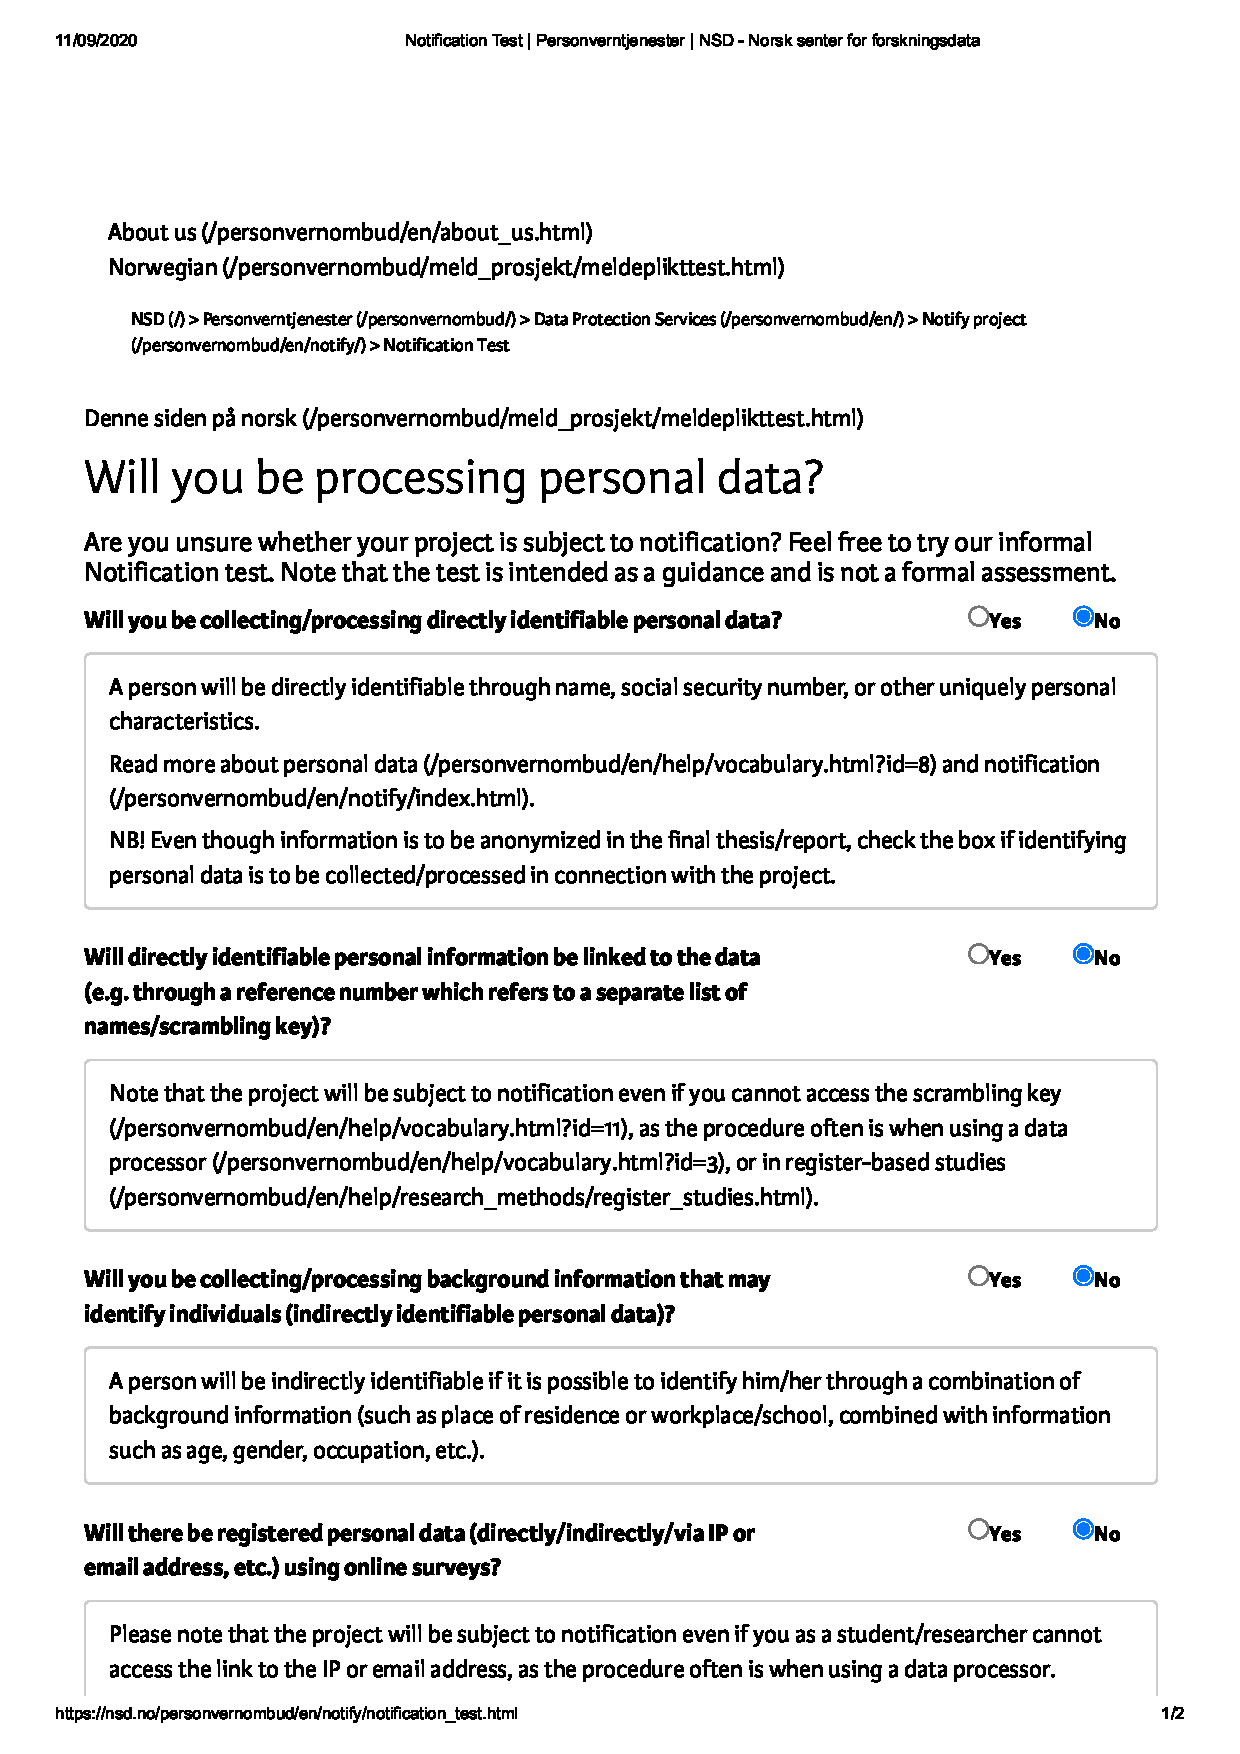
\includepdf[pages=-,fitpaper=true,noautoscale=true]{Appendices/Notification-Test.pdf}


\includepdf[pages=-,fitpaper=true,noautoscale=true]{Appendices/not_subject_to_notification.pdf}


    %\setcounter{secnumdepth}{0}
\chapter{Analysis Code}

\section{Chapter 1}

There is no analysis code in \cref{chp:1}.

\section{Chapter 2}

\subsection{Data Import} \label{R.import}
\begin{singlespace}\small
    \lstinputlisting[language=R,style=vscodeR]{./R/0 Import.R}
\end{singlespace}

\subsection{Missing Pattern Inspection} \label{R.missing}
\begin{singlespace}\small
    \lstinputlisting[language=R,style=vscodeR]{./R/1 Missing.R}
\end{singlespace}

\subsection{Data Reimport} \label{R.reimport}
\begin{singlespace}\small
    \lstinputlisting[language=R,style=vscodeR]{./R/2 Reimport.R}
\end{singlespace}

\subsection{Financial Knowledge Index} \label{R.fki}
\begin{singlespace}\small
    \lstinputlisting[language=R,style=vscodeR]{./R/4 FKI.R}
\end{singlespace}

%     \chapter{Derivation of Country-level Financial Knowledge Indices}

%\epigraph{There are two things you are better off not watching in the making: sausages and\\ econometric estimates.}{Edward Leamer}

\section{Theoretical Foundation}

PISA 2018 financial literacy dataset \parencite{FLdata} provides rich information about students and schools. For the purpose of cross-country comparison, however, the country-level data must be addressed separately by the researchers. \textcite{morenoherrero:2018a}, for instance, introduced a variable ``quality of math and science education'' to control for country-level differences since consensus is yet to emerge about the most appropriate measure for ``countries' financial knowledge''. Inspired by the UN's approach to forming Human Development Indices, a recent publication \textcite{olivermarquez:2020} highlighted four aspects of countries' macroeconomic practices in their attempt to develop country-level financial knowledge indices (FKI).

Oliver-M{\'a}rquez and colleagues consider a country's economic capability, represented by its GDP per capita, to be a key dimension in bringing about its FKI. Secondly, literature converges on the importance of education training for a country's financial knowledge capability \parencite{oecd:2005}. Thirdly, countries with regular engagement with sophisticated financial products and financial markets should possess higher FKI. Lastly, countries with higher aggregate consumption levels and with ageing populations are likely to possess higher FKI due to more frequent exposure and pressure in retirement provision, respetively.

More specifically, \textcite{olivermarquez:2020} suggests using the logarithm of GDP per capital in current international dollars (purchasing power parity adjusted) as a measure for the \texttt{Economic Capability} sub-index. For the \texttt{Education Training} sub-index, the authors consider postgraduate-to-total-tertiary-graduation ratios as a reflection of ``highly skilled'' workforce and the mean years of schooling as a measure of countries' general education levels. For the \texttt{Use} sub-index, gross portfolio equity assets (GPEA) and insurance company assets (ICA) are considered sophisticated financial products countries engage themselves in. Additionally, in order to capture the central role of technology in amplifying the proliferation and use of financial assets, the proportion of Internet users (\textsc{IUS}) enters the definition via
\[ \texttt{Use} = ( \text{GPEA} + \text{ICA} ) ^ \text{IUS}. \]
For the final sub-index \texttt{Need}, the authors define
\[ \texttt{Need} = ( \text{PFA} + \text{AC} ) ^ \text{AGEING}, \]
where \textsc{PFA} is the pension-fund-assets-to-\textsc{GDP} ratio. Aggregate consumption is defined as:
\[ \text{AC} = \frac{2\% \times \text{household final consumption expenditure}}{\text{GDP}}, \]
where the ``$2\%$ rule'' is drawn from \textcite{caliendo:2013} and the proportion of ageing population is computed as
\[ \text{AGEING} = \frac{ \left[ \frac{\text{population}(>65)}{\text{population}(20 \sim 64)} \right]_{2018} - \left[ \frac{\text{population}(>65)}{\text{population}(20 \sim 64)} \right]_{2009} }{ \left[ \frac{\text{population}(>65)}{\text{population}(20 \sim 64)} \right]_{2009} }. \]

\section{Data Collection and Missing Data Treatment}

The data sources for FKI computation are documented in \cref{tab:FKIsource} and its associated notes. The sub-indices \texttt{Educational Training} and \texttt{Use} both contain missing observations for the year 2018. Majority of such missing data appear to be the result of administrative delay, with historic observations available until 2017. It is therefore feasible to conduct time-series forecasts using prior year observations to best approximate 2018 values.

\ltable{tab:FKIsource}{Data Sources for FKI Computation}{
    \begin{tabular}{cclc}
    \toprule
    \multicolumn{1}{c}{Database$\ ^\text{a}$} & Country$\ ^\text{b}$ & \multicolumn{1}{c}{Series} & Time \\
    \midrule
    \rowcolor[rgb]{ .9,  .9,  .9} \multicolumn{4}{c}{Economic Capacity} \\
    WB-dev & 20    & GDP per capita, PPP (current international \$) & 2018 \\
    \rowcolor[rgb]{ .9,  .9,  .9} \multicolumn{4}{c}{Educational Training} \\
    WB-ed & 20 \textbackslash\ Russia & Graduates from ISCED 7 programmes in tertiary education, both sexes (number) & 2013--\textbf{2018} \\
          &       & Graduates from ISCED 8 programmes in tertiary education, both sexes (number) & 2013--\textbf{2018} \\
          &       & Graduates from tertiary education, both sexes (number) & 2013--\textbf{2018} \\
    RS & Russia & PhD (Type 1)$\ ^\text{c}$, PhD (Type 2)$\ ^\text{d}$ & 2018 \\
    RE & Russia & Master (Type 1)$\ ^\text{e}$, Master (Type 2)$\ ^\text{f}$, total tertiary \emph{excluding} PhD$\ ^\text{g}$ & 2018 \\
    HDR & 20    & Dimension = Education; Education = Mean years of schooling (years) & 2018 \\
    \rowcolor[rgb]{ .9,  .9,  .9} \multicolumn{4}{c}{Use} \\
    WB-fin & 20    & Gross portfolio equity assets to GDP (\%) & 2011--\textbf{2018} \\
           &       & Insurance company assets to GDP (\%) & 2011--\textbf{2018} \\
    WB-dev & 20    & Individuals using the Internet (\% of population) & 2009--\textbf{2018} \\
    \rowcolor[rgb]{ .9,  .9,  .9} \multicolumn{4}{c}{Need} \\
    WB-fin & 20 \textbackslash\ Georgia & Pension fund assets to GDP (\%) & 2008--\textbf{2018} \\
    GP & Georgia & Minutes of the meeting of the investment board of the Pension Agency$\ ^\text{h}$ & $\textcolor{white}{\ ^\text{*}}$2019$\ ^\text{*}$ \\
    GS & Georgia & GDP at current prices, billion GEL$\ ^\text{i}$ & 2018 \\
    WB-dev & 20    & Household and NPISHs final consumption expenditure, PPP (current international \$) & 2018 \\
          &       & GDP, PPP (current international \$) & 2018 \\
          &       & Population ages 0--14, male & 2009, 2018 \\
          &       & Population ages 0--14, female & 2009, 2018 \\
          &       & Population ages 15--64, male & 2009, 2018 \\
          &       & Population ages 15--64, female & 2009, 2018 \\
          &       & Population ages 65 and above, male & 2009, 2018 \\
          &       & Population ages 65 and above, female & 2009, 2018 \\
          &       & Population ages 15--19, male (\% of male population) & 2009, 2018 \\
          &       & Population ages 15--19, female (\% of female population) & 2009, 2018 \\
          \bottomrule
    \end{tabular}
}{Sub-indices are shaded in gray. Bold font signifies this year contains missing data.}{3}
\newpage

\begin{singlespace} \small
\begin{itemize}
    \item[$^\text{a}$] WB-dev = \href{https://databank.worldbank.org/source/world-development-indicators}{World Bank -- World development indicators}\\
        WB-ed = \href{https://databank.worldbank.org/source/education-statistics-^-all-indicators}{World Bank -- Education statistics -- All indicators}\\
        WB-fin = \href{https://databank.worldbank.org/source/global-financial-development}{World Bank -- Global financial development}\\
        HDR = \href{http://hdr.undp.org/en/data}{Human Development Reports -- Data}\\
        RS = \href{https://rosstat.gov.ru/}{Russian Federal State Statistic Service}\\
        RE = \href{https://minobrnauki.gov.ru}{Russian Ministry of Education and Science}\\
        GP = \href{https://www.pensions.ge}{Pension Agency of Georgia}\\
        GS = \href{https://www.geostat.ge}{National Statistics Office of Georgia}
    \item[$^\text{b}$] ``20'' = the 20 participating countries in 2018 \textsc{PISA} financial literacy test: Brazil, Bulgaria, Canada, Chile, Estonia, Finland, Georgia, Indonesia, Italy, Latvia, Lithuania, the Netherlands, Peru, Poland, Portugal, Russian Federation, Serbia, Slovak Republic, Spain, and the USA. ``\textbackslash'' = exluding or except
    \item[$^\text{c}$] \href{https://rosstat.gov.ru/storage/mediabank/asp-2(1).xls}{https://rosstat.gov.ru/storage/mediabank/asp-2(1).xls}, Sheet ``\foreignlanguage{russian}{по направлениям подготовки}'', Cell C7 = number of PhD graduates \mbox{(Type 1)}
    \item[$^\text{d}$] \href{https://rosstat.gov.ru/storage/mediabank/asp-3.xls}{https://rosstat.gov.ru/storage/mediabank/asp-3.xls}, Sheet ``\foreignlanguage{russian}{по научным специальностям}'', Cell B7 = number of PhD graduates \mbox{(Type 2)}
    \item[$^\text{e--g}$] \href{https://minobrnauki.gov.ru/common/upload/download/VPO_1_2018.rar}{https://minobrnauki.gov.ru/common/upload/download/VPO{\textunderscore}1{\textunderscore}2018.rar} contains a spreadsheet \textcolor{blue}{\foreignlanguage{russian}{СВОД{\textunderscore}ВПО1{\textunderscore}ВСЕГО}.xls}, Sheet ``P2{\textunderscore}1{\textunderscore}3(1)'', Cell E198 = number of master graduates (Type 1)$^\text{e}$, Cell E410 = number of master graduates (Type 2)$^\text{f}$, Cell E592 = total tertiary graduates \emph{excluding} PhD$^\text{g}$
    \item[$^\text{h}$] \href{https://www.pensions.ge/docs/legislation/investment-board-protocol-4.pdf}{Minutes of the meeting of the investment board of the Pension Agency}, p. 4, no. 3
    \item[$^\text{i}$] \href{https://www.geostat.ge/en/modules/categories/23/gross-domestic-product-gdp}{Gross domestic product (GDP)}, row = GDP at current prices, billion GEL, column = 2018
    \item[$^\text{*}$] Georgia started a \href{https://agenda.ge/en/news/2019/13}{new pension system} on 1 January 2019. Since 2018 was a transitional period with scarce data, 2019 is used as the best approximation for Georgia's pension system for 2018.
\end{itemize}
\end{singlespace}

\clearpage



\subsection{Sub-index \texttt{Educational Training}}

The 2018 archive for the number of master (ISCED 7), PhD (ISCED 8), and total tertiary graduates are incomplete for all participating countries except Georgia, Indonesia and Serbia. \cref{fig:skilled} presents a time series plot of
\[ \texttt{highly skilled} = \frac{\text{number of masters} + \text{number of PhDs}}{\text{total number of tertiary graduates}} \]
and suggests that this ratio is likely to be stable over time, especially between adjacent years. A ``naive forecast'', where the nearest available year's data are to be duplicated for 2018, is applied for \texttt{highly skilled}.

\pfigure{fig:skilled}{Proportion of Postgraduates to Total Tertiary Graduations}{1}{./Figures/skilled.pdf}{``Postgraduate'' is defined as master (ISCED 7) and PhD (ISCED 8) graduates. Countries not shown: GEO, IDN and SRB (2018 data available) and RUS (consult other sources)}{1.75}{1.25}

\subsection{Sub-index \texttt{Use}}

All series involved in calculating this sub-index, GPEA, ICA and IUS, contain missing data. When time series data contain only exponential growth but no underlying trend, a simple exponential smoothing would suffice \parencite{garder:1985}; if trend is present, Holt-Winters method is superior \parencite{chatfield:1978}. \cref{fig:use} facilitates this decision making by plotting both the original and log-transformed versions of GPEA and ICA series. Since curves after log-transformations have slopes, it is prudent to apply the Holt-Winters forecasting method in order to account for possible trends contained in the original series.

\pfigure{fig:use}{Time Series Trend Test}{1}{./Figures/use.pdf}{The time series plots after natural logarithm transformations (bottom panels) are not flat, suggesting the original series (top panels) contain trends. Holt-Winters method therefore is preferred over simple exponential smoothing for 2018 forecasts.}{0.5}{0.85}

The IUS series contains missing data for Canada, Chile and the United States. Similar Holt-Winters procedure is applied to recover 2018 IUS data.

\ltable{tab:FKIraw}{Data Utilised for Computing FKI}{
  \begin{tabular}{cd{3} c d{3}d{1} c d{3}d{3}d{3} c d{3}d{3}d{3}}
    \toprule
    & \multicolumn{1}{c}{Economic Capacity} &       & \multicolumn{2}{c}{Educational Training} &       & \multicolumn{3}{c}{Use} &       & \multicolumn{3}{c}{Need} \\
\cmidrule{2-2}\cmidrule{4-5}\cmidrule{7-9}\cmidrule{11-13}          & \multicolumn{1}{c}{GDP per capita} &       & \multicolumn{1}{c}{Skilled} & \multicolumn{1}{c}{Schooling} &       & \multicolumn{1}{c}{GPEA} & \multicolumn{1}{c}{ICA} & \multicolumn{1}{c}{IUS} &       & \multicolumn{1}{c}{PFA} & \multicolumn{1}{c}{AC} & \multicolumn{1}{c}{AGEING} \\
    \midrule
    BRA   & 9.612 &       & 6.484 & 7.8   &       & 1.683 & 16.259 & 70.434 &       & 11.827 & 1.21  & 0.288 \\
    BGR   & 10.026 &       & 45.294 & 11.8  &       & 4.114 & 7.044 & 64.782 &       & 13.577 & 1.091 & 0.234 \\
    CHL   & 10.117 &       & 16.371 & 10.4  &       & 51.755 & 25.591 & 89.531 &       & 73.225 & 1.073 & 0.214 \\
    EST   & 10.501 &       & 36.765 & 13    &       & 16.399 & 7.681 & 89.357 &       & 18.012 & 0.876 & 0.163 \\
    FIN   & 10.807 &       & 35.024 & 12.4  &       & 93.626 & 31.481 & 88.89 &       & 52.024 & 0.974 & 0.37 \\
    GEO   & 9.588 &       & 24.039 & 12.8  &       & 0.784 & 1.469 & 62.718 &       & 0.834 & 1.227 & 0.042 \\
    IDN   & 9.362 &       & 7.771 & 8     &       & 0.636 & 4.612 & 39.905 &       & 1.826 & 1.059 & 0.145 \\
    ITA   & 10.665 &       & 44.771 & 10.2  &       & 57.434 & 51.26 & 74.387 &       & 10.589 & 1.075 & 0.155 \\
    LVA   & 10.33 &       & 29.554 & 12.8  &       & 8.598 & 2.538 & 83.577 &       & 14.732 & 1.027 & 0.142 \\
    LTU   & 10.487 &       & 28.749 & 13    &       & 9.008 & 5.5   & 79.723 &       & 7.457 & 1.107 & 0.149 \\
    NLD   & 10.961 &       & 32.59 & 12.2  &       & 124.171 & 64.956 & 94.712 &       & 207.938 & 0.805 & 0.326 \\
    PER   & 9.479 &       & 13.577 & 9.2   &       & 16.027 & 6.505 & 52.54 &       & 22.53 & 1.187 & 0.227 \\
    POL   & 10.368 &       & 36.725 & 12.3  &       & 4.853 & 9.535 & 77.542 &       & 9.838 & 1.085 & 0.355 \\
    PRT   & 10.444 &       & 34.454 & 9.2   &       & 19.353 & 25.579 & 74.661 &       & 8.761 & 1.133 & 0.237 \\
    RUS   & 10.267 &       & 30.349 & 12    &       & 0.302 & 2.614 & 80.865 &       & 4.415 & 0.941 & 0.155 \\
    SRB   & 9.774 &       & 26.946 & 11.2  &       & 0.306 & 5.111 & 73.361 &       & 0.845 & 1.171 & 0.28 \\
    SVK   & 10.391 &       & 54.417 & 12.6  &       & 10.644 & 8.873 & 80.66 &       & 12.497 & 0.962 & 0.3 \\
    ESP   & 10.609 &       & 33.929 & 9.8   &       & 27.681 & 28.23 & 86.107 &       & 10.235 & 1.044 & 0.186 \\
    USA   & 11.048 &       & 24.825 & 13.4  &       & 55.505 & 30.183 & 84.881 &       & 150.04 & 1.364 & 0.252 \\
    \bottomrule
    \end{tabular}
}{Full variable names: Skilled = Postgraduate to total tertiary ratio; Schooling = Mean year of schooling; GPEA = Gross portfolio to GDP ratio; ICA = Insurance company assets to GDP ratio; IUS = Number of Internet users per 100 population; PFA = Pension fund assets to GDP ratio; AC = 2\% of household final consumption expenditure to GDP ratio; AGEING = Aged-to-productive-population ratio (\% change between 2009 and 2018)}{3}


\subsection{Other Items with Data Concerns}

Russia reported 67.96\% and 61.01\% of its total university degree receipients to be postgraduates for the year 2013 and 2015 respectively (2014 missing). This figure rapidly declines to 41.6\% in 2016 and further down to 25.69\% in 2017. Such volatility goes against the stable patterns shared by most countries in \cref{fig:skilled}, casting doubt on data reliability. Separate investigation is therefore conducted using Russian government archive (Notes c to g in \cref{tab:FKIsource}).

Georgia underwent pension reform in 2018 with fund balance gradually transitioning to State Pension Agency for its official resumption of duty on 1 January 2019. Resultantly, 2018 pension balance for this country is unavailable but to be best appoximated using 2019 official data (Notes h, i and * of \cref{tab:FKIsource}).

\cref{tab:FKIraw} documents the results of the abovementioned data recovery process.

\section{Standardisation, Weights and FKI}

Following \textcite{olivermarquez:2020}'s procedure, all series in \cref{tab:FKIraw} undergo min-max normalisation such that the smallest entry receives a new score of $0.01$ and the biggest number is re-coded to $0.99$. This slight deviation from the original paper (where the min-max normalisation yields $0$ to $1$) is to avoid multiplying a series by zero or raising a base to the power of zero.

Variable weights are calculated following \textcite{olivermarquez:2020}'s recipe to be the inverses of each series' standard deviations. Whereas a sub-index combines more than one series, each weight is further divided by the sum of the constituent weights so that total weights add to one.

FKI is finally computed by taking the geometric mean of all four sub-indices, subject to sub-index-weights similar to variable weights above, as presented in \cref{tab:FKI}.

\ptable{tab:FKI}{FKI and Sub-indices}{
    \begin{tabular}{c c d{3} c d{3}d{3}d{3}d{3}}
\toprule
        && \multicolumn{1}{c}{FKI}       && \multicolumn{1}{c}{EC}        & \multicolumn{1}{c}{ET}        & \multicolumn{1}{c}{Use}       & \multicolumn{1}{c}{Need}\\
\midrule
        USA   &       & 1.029 &       & 0.990 & 0.590 & 1.467 & 1.580 \\
        ITA   &       & 0.810 &       & 0.767 & 0.601 & 1.603 & 0.767 \\
        ESP   &       & 0.661 &       & 0.734 & 0.464 & 1.012 & 0.670 \\
        LTU   &       & 0.609 &       & 0.664 & 0.633 & 0.325 & 0.801 \\
        PRT   &       & 0.606 &       & 0.639 & 0.401 & 0.869 & 0.719 \\
        CHL   &       & 0.589 &       & 0.449 & 0.302 & 1.372 & 0.939 \\
        EST   &       & 0.576 &       & 0.672 & 0.747 & 0.419 & 0.455 \\
        SVK   &       & 0.552 &       & 0.608 & 0.924 & 0.414 & 0.341 \\
        POL   &       & 0.546 &       & 0.595 & 0.700 & 0.354 & 0.503 \\
        GEO   &       & 0.369 &       & 0.141 & 0.548 & 0.174 & 0.997 \\
        PER   &       & 0.289 &       & 0.078 & 0.194 & 0.780 & 0.868 \\
        BRA   &       & 0.131 &       & 0.155 & 0.010 & 0.506 & 0.809 \\
        IDN   &       & 0.104 &       & 0.010 & 0.040 & 0.975 & 0.734 \\
\bottomrule
    \end{tabular}
}{Table sorted in descending order by countries' FKI. FKI = financial knowledge index, EC = Economic Capability, ET = Educational Training.}{2.5}


%    \chapter{Multilevel Multiple Imputation}
\label{app:MMI}

\section{\textsf{Mplus} Input Code}
\label{sec:MMI_inp}

\lstinputlisting[style=vscodeMplus]{./Mplus/MMI/MMI.inp}

\section{Selected \textsf{Mplus} Output}
\label{sec:MMI_out}

\lstinputlisting[style=vscodeMplus_out,linerange={2909-2967}]{./Mplus/MMI/MMI.out}

\section{Diagnostic Plots}
\label{sec:MMI_diagnostic}

\newpage

% Table generated by Excel2LaTeX from sheet 'Sheet1'
\ltable{tab:MMI}{Summary of Diagnostic Plots of Multilevel Multiple Imputation}{
      \begin{tabular}{ccclrrccc}
\toprule
      Parameter & \multicolumn{1}{c}{Parameter} & Modelling & \multicolumn{1}{c}{Brief} & \multicolumn{1}{c}{Posterior} & \multicolumn{1}{c}{Posterior} & 95\% credibility & Chain & AR-free \\
      number & \multicolumn{1}{c}{label} & level & \multicolumn{1}{c}{description} & \multicolumn{1}{c}{mean} & \multicolumn{1}{c}{variance} & interval & converged & chains \\
\midrule
      1     & \texttt{MALE}  & Within & Whether participant is male & 0.502 &       & (0.499, 0.505) & Yes   & 4 \\
      2     & \texttt{IMMI1GEN} & Within & Whether participant migrated to this country & 0.029 &       & (0.028, 0.030) & Yes   & 4 \\
      3     & \texttt{IMMI2GEN} & Within & Whether their parent did & 0.042 &       & (0.041, 0.044) & Yes   & 4 \\
      4     & \texttt{ESCS}  & Within & Index of economic, social and cultural status & $-$0.241 &       & ($-$0.247, $-$0.234) & Yes   & 4 \\
      5     & \texttt{FCFMLRTY} & Within & Familiarity with concepts of finance & 7.049 &       & (7.015, 7.083) & Yes   & 4 \\
      6     & \texttt{FLCONFIN} & Within & Confidence about financial matters & $-$0.072 &       & ($-$0.079, $-$0.065) & Yes   & 4 \\
      7     & \texttt{FLSCHOOL} & Within & Financial education in school lessons & 0.018 &       & (0.011, 0.024) & Yes   & 4 \\
      8     & \texttt{NOBULLY} & Within & Participant's experience of being bullied (reverse) & $-$0.059 &       & ($-$0.067, $-$0.052) & Yes   & 4 \\
      9     & \texttt{FLFAMILY} & Within & Parental involvement in matters of financial literacy & 0.064 &       & (0.057, 0.070) & Yes   & 4 \\
            &       &       &       &       &       &       &       &  \\
      10    & \texttt{MALE}  & Within & Whether participant is male &       & 0.250 & (0.248, 0.252) & Yes   & 4 \\
      11    & \texttt{IMMI1GEN} & Within & Whether participant migrated to this country &       & 0.028 & (0.028, 0.028) & Yes   & 4 \\
      12    & \texttt{IMMI2GEN} & Within & Whether their parent &       & 0.041 & (0.040, 0.041) & Yes   & 4 \\
      13    & \texttt{ESCS}  & Within & Index of economic, social and cultural status &       & 1.183 & (1.173, 1.193) & Yes   & 4 \\
      14    & \texttt{FCFMLRTY} & Within & Familiarity with concepts of finance &       & 29.754 & (29.495, 30.016) & Yes   & 4 \\
      15    & \texttt{FLCONFIN} & Within & Confidence about financial matters &       & 1.034 & (1.025, 1.044) & Yes   & 4 \\
      16    & \texttt{FLSCHOOL} & Within & Financial education in school lessons &       & 1.040 & (1.031, 1.049) & Yes   & 4 \\
      17    & \texttt{NOBULLY} & Within & Participant's experience of being bullied (reverse) &       & 1.111 & (1.100, 1.121) & Yes   & 4 \\
      18    & \texttt{FLFAMILY} & Within & Parental involvement in matters of financial literacy &       & 1.090 & (1.080, 1.100) & Yes   & 4 \\
            &       &       &       &       &       &       &       &  \\
      19    & \texttt{STRAIO} & Between & Student$-$teacher ratio & 13.873 &       & (13.607, 14.139) & Yes   & 4 \\
      20    & \texttt{EDUSHORT} & Between & Shortage of educational material & 0.131 &       & (0.106, 0.157) & Yes   & 4 \\
            &       &       &       &       &       &       &       &  \\
      21    & \texttt{STRAIO} & Between & Student$-$teacher ratio &       & 103.532 & (99.750, 107.430) & Yes   & 4 \\
      22    & \texttt{EDUSHORT} & Between & Shortage of educational material &       & 1.074 & (1.037, 1.112) & Yes   & 4 \\
\bottomrule
      \end{tabular}
}{Notes go here.}{6}
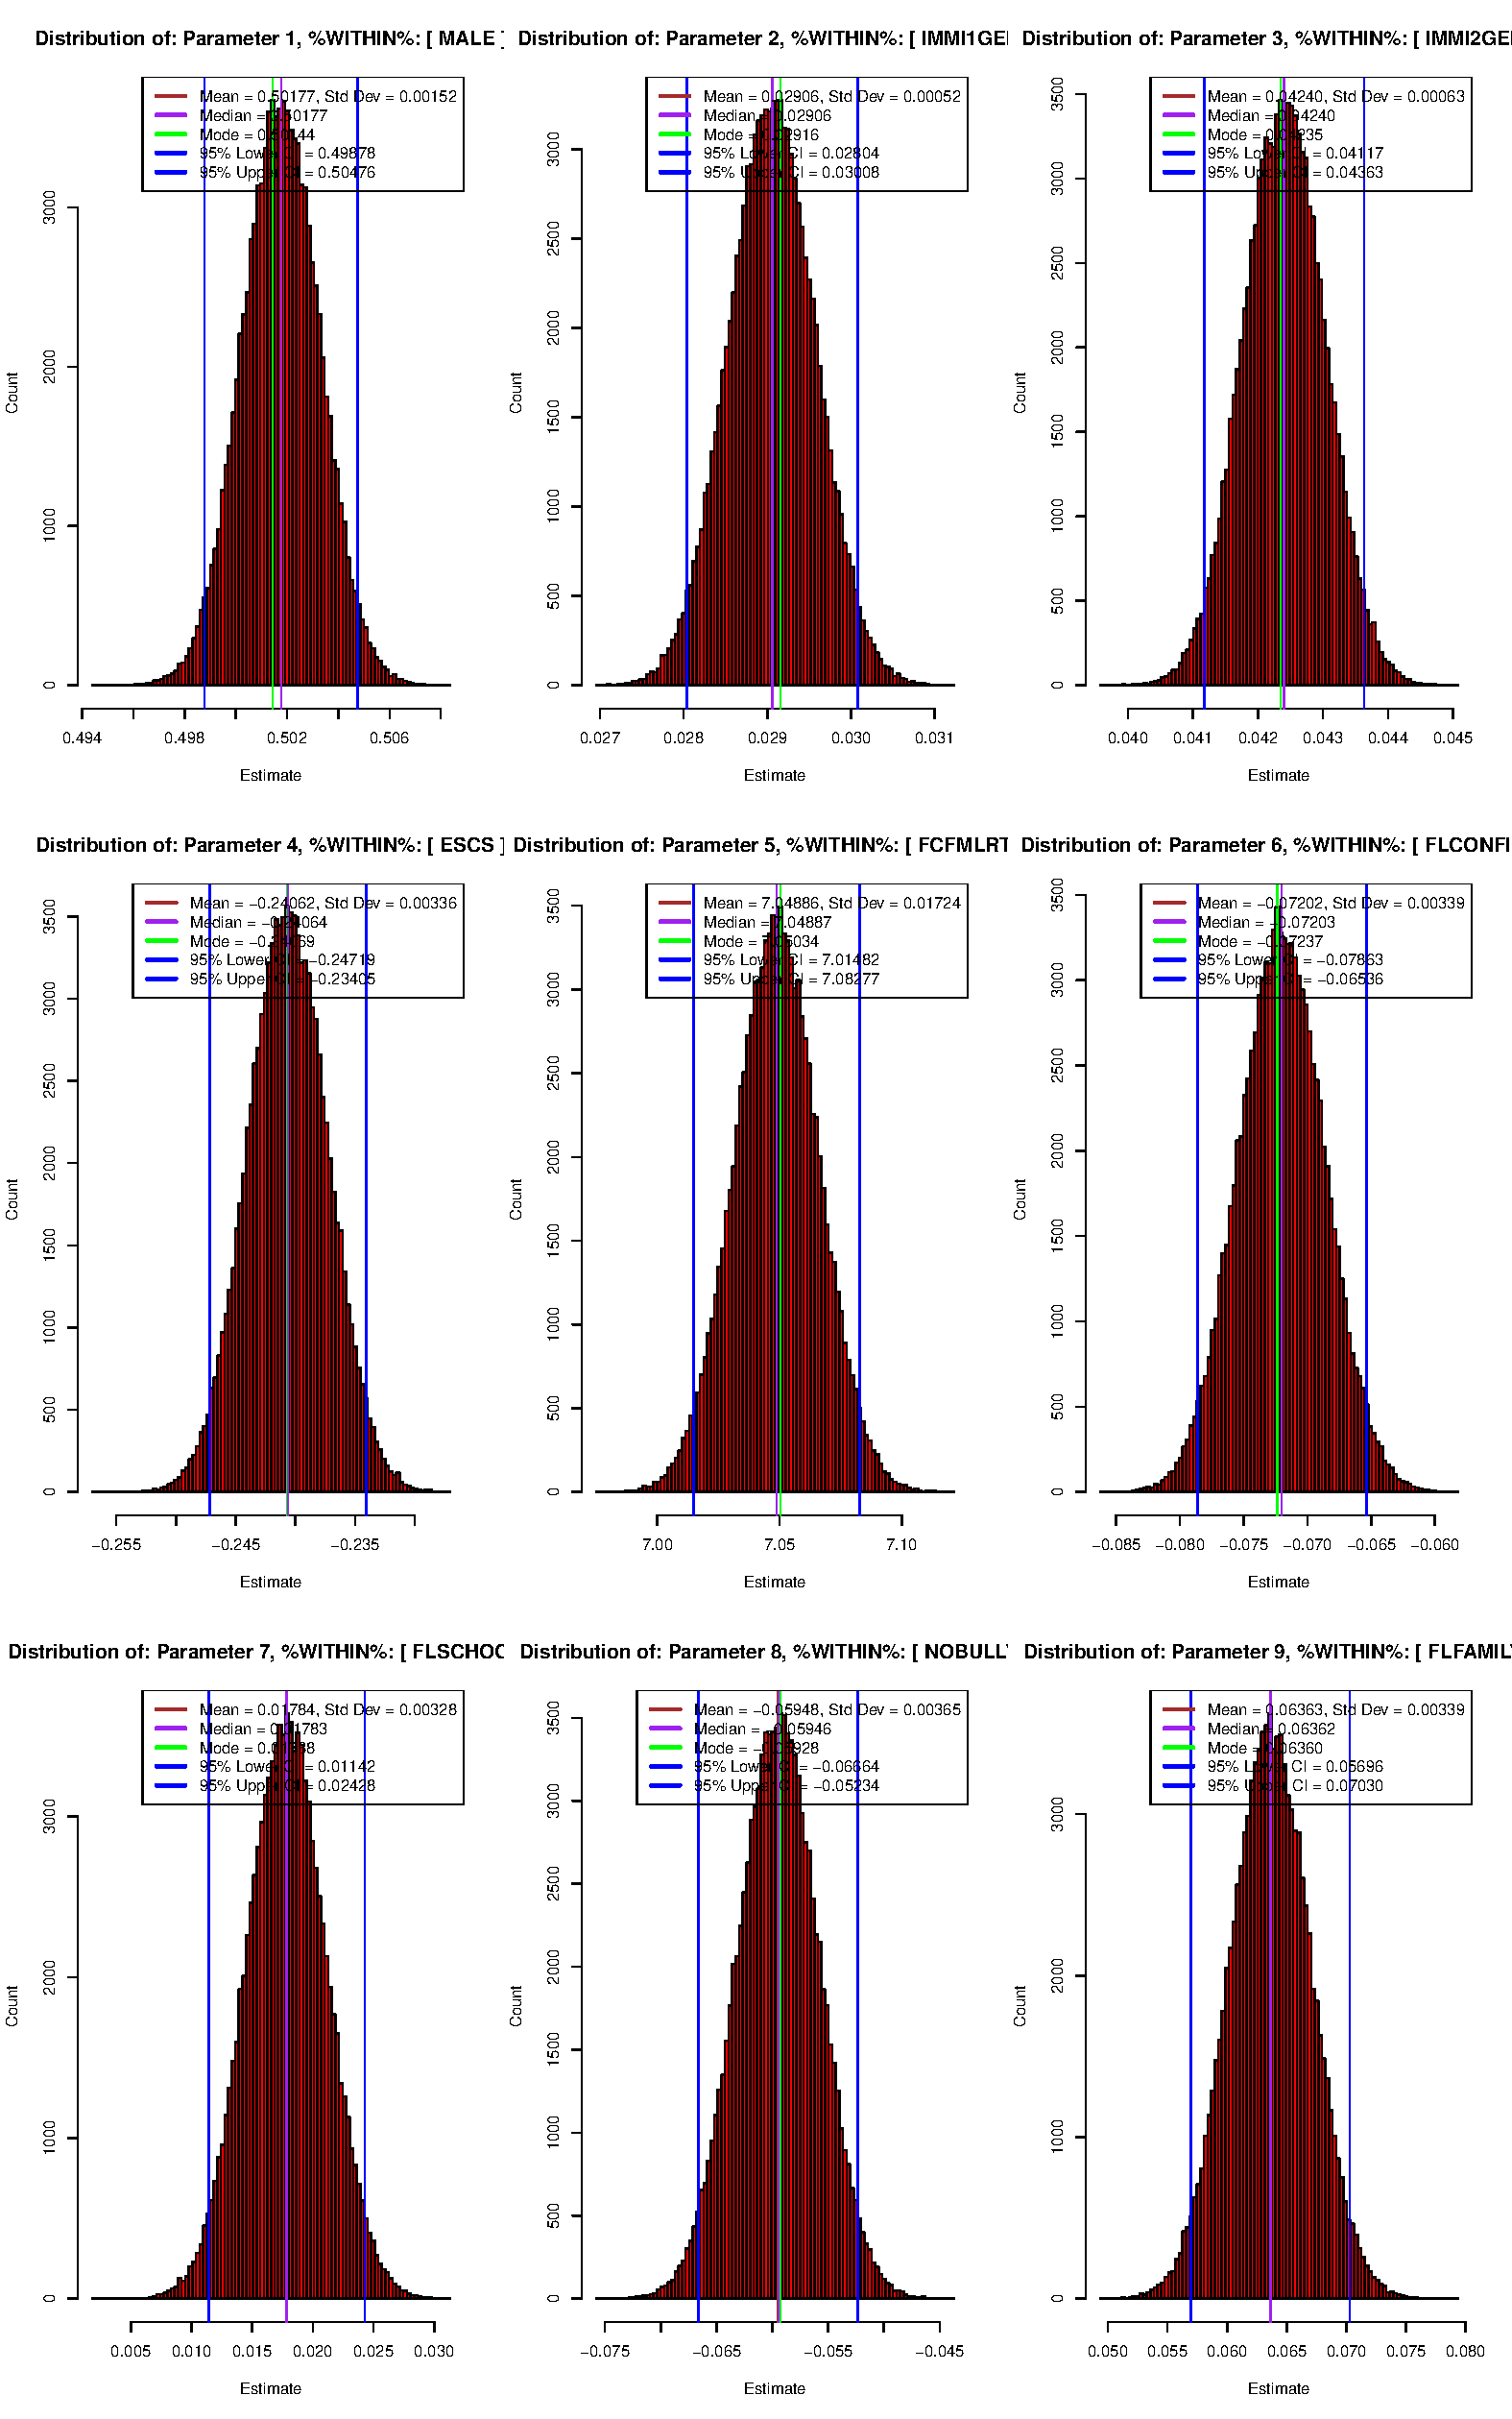
\includepdf[pages=-,width=\textwidth]{./Figures/MMI_diagnostic.pdf}

%    \include{Appendices/E}
%    \include{Appendices/F}
%    \chapter[Derivation of Moderated Mediation Effect]{Derivation of Moderated\\Mediation Effect}

\section{Models with Mediators Only}

Consider a SEM model 
%with three independent variables ($X_1$, $X_2$ and $X_3$) and two mediators ($M_1$ and $M_2$) as
shown in \cref{fig:moderator} (excluding any paths in green), where
\begin{equation*}
    \left\{
    \begin{aligned}
        Y &= \mu_0 + b_1M_1 + b_2M_2 + c_1X_1 + c_2X_2 + c_3X_3\\
        M_1 &= \mu_1 + a_{11}X_1 + a_{21}X_2 + a_{31}X_3\\
        M_2 &= \mu_2 + a_{12}X_1 + a_{22}X_2 + a_{32}X_3
    \end{aligned}
    \right.
\end{equation*}
or, in matrix form
\begin{equation}
    \left\{
    \begin{aligned}
        Y &= \mu_0 + \T{b}\m{m} + \T{c}\m{x}\\
        \m{m} &= \m{\mu} + \T{A}\m{x}
    \end{aligned}
    \right.
\end{equation}
where
\begin{equation*}\label{eq:0}
    \md{x}{3}{1} =
        \begin{bmatrix}
            X_1\\
            X_2\\
            X_3
        \end{bmatrix},\ 
    \md{m}{2}{1} =
        \begin{bmatrix}
            M_1\\
            M_2
        \end{bmatrix},\ 
    \md{b}{2}{1} =
        \begin{pmatrix}
            b_1\\
            b_2
        \end{pmatrix},\ 
    \md{c}{3}{1} =
        \begin{pmatrix}
            c_1\\
            c_2\\
            c_3
        \end{pmatrix},\ 
    \md{\mu}{2}{1} =
        \begin{pmatrix}
            \mu_1\\
            \mu_2
        \end{pmatrix}\text{and}\ 
    \md{A}{3}{2} =
        \begin{pmatrix}
            a_{11}    &a_{12}\\
            a_{21}    &a_{22}\\
            a_{31}    &a_{32}
        \end{pmatrix}
\end{equation*}

\cref{eq:0} can be written as a total equation:
\begin{equation}\label{eq:tot0}
    Y = \mu_0 + \T{b}\m{\mu} + \T{b}\T{A}\m{x} + \T{c}\m{x} = \left( \mu_0 + \T{b}\m{\mu} \right) + \T{x} \left( \m{A}\m{b} + \m{c} \right)
\end{equation}
where $\mu_0 + \T{b}\m{\mu}$ is the intercept, $\m{A}\m{b}$ is the indirect effect and $\m{c}$ is the direct effect.

\section{Models with Moderated Mediators}

Now introduce two moderators $D_1$ and $D_2$ (green paths in \cref{fig:moderator}).

In scalar notation:
\begin{equation*}
    \begin{aligned}
        Y_\text{mod} &= \mu_0 + b_1M_1 + b_2M_2 + c_1X_1 + c_2X_2 + c_3X_3\\
        &+ f_1D_1 + f_2D_2\\
        &+ g_{11}X_1D_1 + g_{12}X_1D_2\\
        &+ g_{21}X_2D_1 + g_{22}X_2D_2\\
        &+ g_{31}X_3D_1 + g_{32}X_1D_2\\
        &+ h_{11}M_1D_1 + h_{12}M_1D_2\\
        &+ h_{21}M_2D_1 + h_{22}M_2D_2
    \end{aligned}
\end{equation*}
and in matrix notation:
\begin{equation}\label{eq:mod}
    Y_\text{mod} = \mu_0 + \T{b}\m{m} + \T{c}\m{x} + \T{f}\m{d} + \tr{\T{G}\m{x}\T{d}} + \tr{\T{H}\m{m}\T{d}}
\end{equation}
where,
\begin{equation*}
    \md{f}{2}{1} =
        \begin{pmatrix}
            f_1\\
            f_2
        \end{pmatrix},\ 
    \md{d}{2}{1} =
        \begin{bmatrix}
            D_1\\
            D_2
        \end{bmatrix},\ 
    \md{G}{3}{2} =
        \begin{pmatrix}
            g_{11}  &g_{12}\\
            g_{21}  &g_{22}\\
            g_{31}  &g_{32}
        \end{pmatrix},\ 
    \md{H}{2}{2} =
    \begin{pmatrix}
        h_{11}  &h_{12}\\
        h_{21}  &h_{22}
    \end{pmatrix},
\end{equation*}
and $\tr{\cdot}$ is the trace operator.

Since $\m{m} = \m{\mu} + \T{A}\m{x}$, \cref{eq:mod} can be expanded into:
\begin{equation}\label{eq:totmod}
    \begin{aligned}
        Y_\text{mod} &= \mu_0 + \T{b}\m{\mu} + \T{b}\T{A}\m{x} + \T{c}\m{x} + \T{f}\m{d} + \tr{\T{G}\m{x}\T{d}} + \tr{\T{H}\m{\mu}\T{d}} + \tr{\T{H}\T{A}\m{x}\T{d}}\\
        &= \left[ \mu_0 + \T{b}\m{\mu} + \T{f}\m{d} + \tr{\T{H}\m{\mu}\T{d}} \right] + \left[ \left( \T{b}\T{A} + \T{c} \right) \m{x} + \tr{\T{d}\left( \T{G} + \T{H}\T{A} \right) \m{x}} \right]\\
        &= \left[ \mu_0 + \T{b}\m{\mu} + \T{f}\m{d} + \tr{\T{H}\m{\mu}\T{d}} \right] + \left[ \left( \T{b}\T{A} + \T{c} \right) \m{x} + \T{d}\left( \T{G} + \T{H}\T{A} \right) \m{x} \right]\\
        &= \left[ \mu_0 + \T{b}\m{\mu} + \T{f}\m{d} + \tr{\T{H}\m{\mu}\T{d}} \right] + \T{x} \left[ \m{A}\m{b} + \m{c} + \m{G}\m{d} + \m{A}\m{H}\m{d} \right]\\
        &= \left[ \mu_0 + \T{b}\m{\mu} + \T{f}\m{d} + \tr{\T{H}\m{\mu}\T{d}} \right] + \T{x} \left[ \m{A} \left( \m{b} + \m{H}\m{d} \right) + \left( \m{c} + \m{G}\m{d} \right) \right]
    \end{aligned}
\end{equation}

\cref{eq:totmod} differs from \cref{eq:tot0} by one extra term $\m{f}\T{d} + \tr{\T{H}\m{\mu}\T{d}}$ in the intercept. The indirect effect $\m{A}\m{b}$ expanded to $\m{A} \left( \m{b} + \m{H}\m{d} \right)$ as a result of introducing the moderators and the direct effect grows from $\m{c}$ to $\m{c} + \m{G}\m{d}$.

\newpage

Expand the indirect and direct effects back to their scalar forms:

\begin{equation*}
    \begin{aligned}
        &\text{indirect effects}\\
        = &\m{A} \left( \m{b} + \m{H}\m{d} \right)\\
        = &\begin{pmatrix}
            a_{11}    &a_{12}\\
            a_{21}    &a_{22}\\
            a_{31}    &a_{32}
        \end{pmatrix}
        \left[\begin{pmatrix}
            b_1\\
            b_2
        \end{pmatrix} +
        \begin{pmatrix}
            h_{11}  &h_{12}\\
            h_{21}  &h_{22}
        \end{pmatrix}
        \begin{bmatrix}
            D_1\\
            D_2
        \end{bmatrix}
        \right]\\
        = &\begin{pmatrix}
            a_{11}    &a_{12}\\
            a_{21}    &a_{22}\\
            a_{31}    &a_{32}
        \end{pmatrix}
        \begin{pmatrix}
            b_1 + h_{11}D_1 + h_{12}D_2\\
            b_2 + h_{21}D_1 + h_{22}D_2
        \end{pmatrix}\\
        = &\begin{pmatrix}
            a_{11}b_1 + a_{11}h_{11}D_1 + a_{11}h_{12}D_2 +
            a_{12}b_2 + a_{12}h_{21}D_1 + a_{12}h_{22}D_2\\
            a_{21}b_1 + a_{21}h_{11}D_1 + a_{21}h_{12}D_2 +
            a_{22}b_2 + a_{22}h_{21}D_1 + a_{22}h_{22}D_2\\
            a_{31}b_1 + a_{31}h_{11}D_1 + a_{31}h_{12}D_2 +
            a_{32}b_2 + a_{32}h_{21}D_1 + a_{32}h_{22}D_2
        \end{pmatrix};\\
        &\text{direct effects}\\
        = &\m{c} + \m{G}\m{d}\\
        = &\begin{pmatrix}
            c_1\\
            c_2\\
            c_3
        \end{pmatrix} +
        \begin{pmatrix}
            g_{11}  &g_{12}\\
            g_{21}  &g_{22}\\
            g_{31}  &g_{32}
        \end{pmatrix}
        \begin{bmatrix}
            D_1\\
            D_2
        \end{bmatrix}\\
        = &\begin{pmatrix}
            c_1 + g_{11}D_1 + g_{12}D_2\\
            c_2 + g_{21}D_1 + g_{22}D_2\\
            c_3 + g_{31}D_1 + g_{32}D_2
        \end{pmatrix}.
    \end{aligned}
\end{equation*}

\section{Mplus Execution}

The \texttt{DEFINE:} and \texttt{MODEL:} sections of the Mplus code is given as following:

\begin{singlespace}\tiny
    \begin{lstlisting}
DEFINE:

    ! G matrix
    X1D1 = X1 * D1;
    X2D1 = X2 * D1;
    X3D1 = X3 * D1;
    X1D2 = X1 * D2;
    X2D2 = X2 * D2;
    X3D2 = X3 * D2;
    ! H matrix
    M1D1 = M1 * D1;
    M2D1 = M2 * D1;
    M1D2 = M1 * D2;
    M2D2 = M2 * D2;

MODEL:

    [Y] (mu0);
    Y on M1 (b1);
    Y on M2 (b2);
    ! ---
    Y on M1D1 (h11);
    Y on M2D1 (h21);
    Y on M1D1 (h12);
    Y on M2D1 (h22);
    ! ---
    Y on X1 (c1);
    Y on X2 (c2);
    Y on X3 (c3);
    ! ---
    Y on D1 (f1);
    Y on D2 (f2);
    ! ---
    Y on X1D1 (g11);
    Y on X2D1 (g21);
    Y on X3D1 (g31);
    Y on X1D2 (g12);
    Y on X2D2 (g22);
    Y on X3D2 (g32);

    [M1] (mu1);
    M1 on X1 (a11);
    M1 on X2 (a21);
    M1 on X3 (a31);

    [M2] (mu2);
    M2 on X1 (a12);
    M2 on X2 (a22);
    M2 on X3 (a32);
    \end{lstlisting}
\end{singlespace}

\ltikz{fig:moderator}{Moderated Mediation Model}{
\begin{tikzpicture}[
    manvar/.style={rectangle,draw=black,minimum width=1.5cm},
    ->,>=stealth',semithick,
    bend angle=-45,
    decoration={
        zigzag,
        amplitude=1pt,
        segment length=1mm,
        post=lineto,
        post length=4pt
    }
]

% MODEL DIAGRAM

% Draw independent vars (X)
    \node[manvar] (0X1) at (1,9) {$X_1$};
    \node[manvar] (0X2) at (1,6) {$X_2$};
    \node[manvar] (0X3) at (1,3) {$X_3$};

% Draw mediators (M)
    \node[manvar] (0M1) at (4,7) {$M_1$};
    \node[manvar] (0M2) at (4,5) {$M_2$};

% Draw moderators (D)
    \node[manvar] (0D1) at (7,8) {$D_1$};
    \node[manvar] (0D2) at (7,4) {$D_2$};

% Draw dependent var (Y)
    \node[manvar] (0Y) at (10,6) {$Y$};

% Link X with M
    \draw[blue,->] (0X1.east) to node[above,sloped,pos=0.5] {$a_{11}$} (0M1.west);
    \draw[blue,->] (0X2.east) to node[] {} (0M1.west);
    \draw[blue,->] (0X3.east) to node[] {} (0M1.west);

    \draw[blue,->] (0X1.east) to node[] {} (0M2.west);
    \draw[blue,->] (0X2.east) to node[] {} (0M2.west);
    \draw[blue,->] (0X3.east) to node[below,sloped,pos=0.5] {$a_{32}$} (0M2.west);

% Link M with Y
    \draw[blue,->] (0M1.east) to node[above,sloped] {$b_1$} (0Y.west);
    \draw[blue,->] (0M2.east) to node[below,sloped] {$b_2$} (0Y.west);

% Link X with Y
    \draw[red,->] (0X1.east) to node[above,sloped,pos=0.3] {$c_1$} (0Y.west);
    \draw[red,->] (0X2.east) to node[pos=0.3] {$c_2$} (0Y.west);
    \draw[red,->] (0X3.east) to node[below,sloped,pos=0.3] {$c_3$} (0Y.west);

% Moderate on direct pathways
    \draw[forestgreen,->] (6.25,8)--(5.5,7.5);
    \draw[forestgreen,->] (6.25,8)--(5.5,6);
    \draw[forestgreen,->] (6.25,8)--(5.5,4.5);

    \draw[forestgreen,->] (6.25,4)--(5.5,7.5);
    \draw[forestgreen,->] (6.25,4)--(5.5,6);
    \draw[forestgreen,->] (6.25,4)--(5.5,4.5);

% Moderate on indirect pathways
    \draw[forestgreen,->] (7,7.7)--(8.5,6.17);
    \draw[forestgreen,->] (7,7.7)--(8.5,5.83);

    \draw[forestgreen,->] (7,4.3)--(8.5,6.17);
    \draw[forestgreen,->] (7,4.3)--(8.5,5.83);


% STATISTICAL DIAGRAM

% Draw independent vars (X)
    \node[manvar] (X1) at (0,0) {$X_1$};
    \node[manvar] (X2) at (0,-1) {$X_2$};
    \node[manvar] (X3) at (0,-2) {$X_3$};

% Draw mediators (M)
    \node[manvar] (M1) at (3,-4) {$M_1$};
    \node[manvar] (M2) at (3,-5) {$M_2$};

% Draw dependent var (Y)
    \node[manvar] (Y) at (7,-3) {$Y$};

% Draw moderators (D)
    \node[manvar] (D1) at (7,1) {$D_1$};
    \node[manvar] (D2) at (9,1) {$D_2$};

% Draw X * D interactions
    \node[manvar] (X1D1) at (11,0) {$X_1D_1$};
    \node[manvar] (X2D1) at (11,-1) {$X_2D_1$};
    \node[manvar] (X3D1) at (11,-2) {$X_3D_1$};

    \node[manvar] (X1D2) at (13,0) {$X_1D_2$};
    \node[manvar] (X2D2) at (13,-1) {$X_2D_2$};
    \node[manvar] (X3D2) at (13,-2) {$X_3D_2$};

% Draw M * D interactions
    \node[manvar] (M1D1) at (11,-4) {$M_1D_1$};
    \node[manvar] (M2D1) at (11,-5) {$M_2D_1$};

    \node[manvar] (M1D2) at (13,-4) {$M_1D_2$};
    \node[manvar] (M2D2) at (13,-5) {$M_2D_2$};

% Link X with M (a)
    \draw[blue,->] (X1.east) to node[above,sloped,pos=0.7] {$a_{11}$} (M1.west);
    \draw[blue,->] (X1.east) to node[above,sloped] {} (M2.west);

    \draw[blue,->] (X2.east) to node[above,sloped] {} (M1.west);
    \draw[blue,->] (X2.east) to node[above,sloped] {} (M2.west);

    \draw[blue,->] (X3.east) to node[above,sloped] {} (M1.west);
    \draw[blue,->] (X3.east) to node[below,sloped,pos=0.4] {$a_{32}$} (M2.west);

% Link M with Y (b)
    \draw[blue,->] (M1.east) to node[above,sloped,pos=0.4] {$b_1$} (Y.west);
    \draw[blue,->] (M2.east) to node[below,sloped,pos=0.4] {$b_2$} (Y.west);

% Link X with Y (c)
    \draw[red,->] (X1.east) to node[above,sloped] {$c_1$} (Y.west);
    \draw[red,->] (X2.east) to node[above,sloped] {} (Y.west);
    \draw[red,->] (X3.east) to node[below,sloped] {$c_3$} (Y.west);

% Link D with Y (f)
    \draw[forestgreen,->] (D1.south) to node[below,sloped,rotate=180,pos=0.3] {$f_1$} (Y.north);
    \draw[forestgreen,->] (D2.south) to node[above,sloped,pos=0.4] {$f_2$} (Y.north);

% Link XD with Y (G)
    \draw[forestgreen,->] (X1D1.west) to node[below,sloped] {$g_{11}$} (Y.east);
    \draw[forestgreen,->] (X3D2.west) to node[above,sloped,pos=0.6] {$g_{32}$} (Y.east);

% Link MD with Y (H)
    \draw[forestgreen,->] (M1D1.west) to node[above,sloped,pos=0.4] {$h_{11}$} (Y.south);
    \draw[forestgreen,->] (M2D2.west) to node[below,sloped,pos=0.65] {$h_{22}$} (Y.south);
\end{tikzpicture}
}{A moderated mediation is shown in both model diagram (upper panel) and statistical diagram (lower panel). \textcolor{red}{Direct paths}, \textcolor{blue}{indirect paths} and \textcolor{forestgreen}{moderations} are differentiated by colour.}

%    \chapter{Review of Matrix Calculus}

\section{Notations}

Let us first establish the notation. This is important because bad notation is a serious obstacle to elegant mathematics and coherent exposition and it can be misleading.

Unless specified otherwise, $\phi$ denotes a scalar function; $\m{f}$ a vector function and $\m{F}$ a matrix function. Also, $x$ denotes a scalar argument, $\m{x}$ a vector argument and $\m{X}$ a matrix argument. For example, we write

\begin{table*}[h]
  \begin{center}
  \begin{tabular}{lll}
    $\phi(x)=x^2$     &$\phi(\m{x})=\T{a}\m{x}$       &$\phi(\m{X})=\tr{\T{X}\m{X}}$\\
    $\m{f}(x)=
      \begin{pmatrix}
        x\\
        x^2
      \end{pmatrix}$    &$\m{f}(\m{x})=\m{Ax}$    &$\m{f}(\m{X})=\m{Xa}$\\
      $\m{F}(x)=x^2\Id{m}$  &$\m{F}(\m{x})=\m{x}\T{x}$  &$\m{F}(\m{X})=\T{X}$
  \end{tabular}
\end{center}
\end{table*}

Since the prime notation $'$ may easily cause confusion between derivatives and transposes, preference is given to the Leibniz notation $\frac{\dd}{\dd x}$ for derivatives and $\T{}$ for transposes---unless this system becomes too cumbersome, in which case $\m{f}'(\m{x})$ will denote derivatives and $\m{f}(\m{x})'$ for transposes.

\section{Derivatives and differentials}

\subsection{Derivative}

\theoremstyle{definition}
\begin{definition}[Derivatives]\label{Def.D}
  If $\m{f}$ is an $m\times 1$ vector function of an $n\times 1$ vector $\m{x}$, then the \emph{derivative} (or \emph{Jacobian matrix}) of $\m{f}$ is the $m\times n$ matrix
  \begin{equation}\label{Eq.Def.D}
    \D\m{f}(\m{x}):=\frac{\partial\m{f}(\m{x})}{\partial\T{x}},
  \end{equation}
  whose elements are the partial derivatives
  \begin{equation*}
    \frac{\partial f_i(\m{x})}{\partial x_j},\ \text{for}\ %
    \begin{aligned}
      i&=1,\cdots,m,\\
      j&=1,\cdots,n.
    \end{aligned}
  \end{equation*}
\end{definition}

\subsection{Differential}

In the one dimensional case, the equation
\begin{equation}\label{Eq.D}
  \lim_{u\to 0}\frac{\phi(x+u)-\phi(x)}{u}=\phi'(x)
\end{equation}
defines the derivative of $\phi$ at $x$. Rewriting \cref{Eq.D} gives
\begin{equation}\label{Eq.d}
  \phi(x+u)=\phi(x)+\phi'(x)u+O(u),
\end{equation}
where the remainder term $O(u)$ quickly vanishes as $u$ approaches $0$.

\theoremstyle{definition}
\begin{definition}[Differential]
  We define the (first) \emph{differential} of $\phi$ at $x$ (with increment $u$) as
  \begin{equation}
    \dd\phi(x;u)=\phi'(x)u.
  \end{equation}
\end{definition}

For example, for $\phi(x)=x^2$, we have $\dd\phi(x;u)=2xu$. In practice, we write $\dd x$ instead of $u$, so that $\dd\phi(x)=\phi'(x)\dd x=2x\dd x.$

In the vector case, similar to \cref{Eq.d}, we have
\begin{equation}
  \m{f}(\m{x}+\m{u})=\m{f}(\m{x})+[\D\m{f}(x)]\m{u}+O(\m{u}),
\end{equation}
and the (first) differential is defined as
\begin{equation}
  \dd\m{f}(\m{x};\m{u})=[\D\m{f}(x)]\m{u}.
\end{equation}

Although rarely used in econometrics, for completeness, the matrix case can be obtained from the vector case by writing $\m{f}:=\vec{F}$ and $\m{x}:=\vec{X}$.

\subsection{Which to use?}

For practical rather than theoretical reasons, the treatment of matrix calculus is based on differentials ($\dd\m{f}$) rather than derivatives ($\D\m{f}$) because the former yields a result with the same dimension as $\m{f}$. For example, consider $\md{f}{m}{1}(\md{x}{n}{1})$ (reading ``$\m{f}$ being an $m\times 1$ vector function of an $n\times 1$ vector $\m{x}$''), $\D\m{f}(\m{x})$ is an $m\times n$ matrix (due to \cref{Def.D}) whereas $\dd\m{f}(\m{x})$ remains an $m\times 1$ vector (same as $\m{f}$). The advantage is even larger for matrices: for $\md{F}{m}{p}(\md{X}{n}{q})$, $\dd\m{F}(\m{X})$ has the same dimension as $\m{F}$ irrespective of the dimension of $\m{X}$, but $\D\m{F}(\m{X})$ is going to be a horrendous $mp\times nq$ matrix.

\section{Layout convention}\label{S.layout}

Under the \emph{numerator layout}, when we differentiate a scalar function $\phi$ \wrt a column vector $\md{x}{n}{1}$, we get a \emph{row} vector of dimension $1\times n$. If we want our result to be in the column form, we must differentiate $\phi$ \wrt a row vector to start with. This is why the denominator in \cref{Eq.Def.D} contains a transpose.

\section{Application in OLS}

\subsection{Background}

Imagine we are interested in learning the return on education. We might propose a rather simple model
\begin{equation}
  \texttt{inc}=\beta_0+\beta_1\texttt{edu}+\beta_2\texttt{exp}+\epsilon
\end{equation}
where \texttt{inc} is one's income, \texttt{edu} and \texttt{exp} denote years of formal education and years spent in the labour market, respectively.

We managed to collect survey data from $n$ respondents and organised this information in the following system of equations:
\begin{equation}
  \left\{
    \begin{aligned}
      \texttt{inc}_1 &= \beta_0+\beta_1\texttt{edu}_1+\beta_2\texttt{exp}_1+\epsilon_1\\
      \texttt{inc}_2 &= \beta_0+\beta_1\texttt{edu}_2+\beta_2\texttt{exp}_2+\epsilon_2\\
      \cdots\\
      \texttt{inc}_n &= \beta_0+\beta_1\texttt{edu}_n+\beta_2\texttt{exp}_n+\epsilon_n\\
    \end{aligned}
  \right.
\end{equation}

This system of linear equations can be represented in the matrix notation using
\begin{equation}
  \md{y}{n}{1}=
    \begin{pmatrix}
      \texttt{inc}_1\\
      \texttt{inc}_2\\
      \cdots\\
      \texttt{inc}_2\\
    \end{pmatrix},\ %
  \md{X}{n}{3}=
    \begin{pmatrix}
      1     &\texttt{edu}_1     &\texttt{exp}_1\\
      1     &\texttt{edu}_2     &\texttt{exp}_2\\
      \cdots\\
      1     &\texttt{edu}_n     &\texttt{exp}_n\\
    \end{pmatrix},\ %
  \md{\beta}{3}{1}=
    \begin{pmatrix}
      \beta_0\\
      \beta_1\\
      \beta_2\\
    \end{pmatrix},\ \text{and}\ %
  \md{\epsilon}{n}{1}=
    \begin{pmatrix}
      \epsilon_1\\
      \epsilon_2\\
      \cdots\\
      \epsilon_n\\
    \end{pmatrix}
  \end{equation}
as
\begin{equation}\label{Eq.setup}
  \m{y}=\m{X\beta}+\m{\epsilon}.
\end{equation}

\subsection{Ordinary least squares}

The objective of OLS is to minimise the \emph{sum of squared} error terms. A handy way of representing sum of squared $\epsilon$ is
\begin{equation}
  \text{SSE}=\sum_{i=1}^n\epsilon_i^2=\epsilon_1^2+\epsilon_2^2+\cdots+\epsilon_n^2=
  \begin{pmatrix}
    \epsilon_1      &\epsilon_2     &\cdots      &\epsilon_n
  \end{pmatrix}
  \begin{pmatrix}
    \epsilon_1\\
    \epsilon_2\\
    \cdots\\
    \epsilon_n
  \end{pmatrix}
  =\T{\epsilon}\m{\epsilon}.
\end{equation}
In fact, $\T{x}\m{x}$ is the mathematical translation of ``sum of squared'' of $\m{x}$.

Now we are ready to continue. We want to carefully choose a combination of $\beta_0$, $\beta_1$ and $\beta_2$ in order to make SSE as small as possible, ie
\begin{equation}\label{Eq.min}
  \min{\T{\epsilon}\m{\epsilon}}{\m{\beta}}=\min{\left(\m{y}-\m{X\beta}\right)\Ts\left(\m{y}-\m{X\beta}\right)}{\m{\beta}}
\end{equation}
(the equal sign is due to \cref{Eq.setup}).

Two observations can be made from the minimisation problem in \cref{Eq.min}:
\begin{enumerate}
  \item both $\m{y}$ and $\m{X}$ are collected data therefore can no longer be changed by the researcher; but we are free to adjust $\m{\beta}$ in whatever way we want, meaning $\m{\beta}$ is the ``independent variable'' and SSE is a function of $\m{\beta}$, and
  \item $\T{\epsilon}\m{\epsilon}$ is a scalar function (please verify).
\end{enumerate}
Then,
\begin{equation}
  \begin{aligned}
    \phi(\m{\beta})=\T{\epsilon}\m{\epsilon}&=\left(\m{y}-\m{X\beta}\right)\Ts\left(\m{y}-\m{X\beta}\right)\\
  &=\left(\T{y}-\T{\beta}\T{X}\right)\left(\m{y}-\m{X\beta}\right)\\
  &=\T{y}\m{y}-\T{y}\m{X\beta}-\T{\beta}\T{X}\m{y}+\T{\beta}\T{X}\m{X\beta}
  \end{aligned}
\end{equation}

We now differentiate $\phi(\m{\beta})$ \wrt $\m{\beta}$:
\begin{equation}\label{Eq.normal}
  \begin{aligned}
    \frac{\dd \phi(\m{\beta})}{\dd\m{\beta}}&=-\T{y}\m{X}-\frac{\dd}{\dd\m{\beta}}\left[\left(\T{\beta}\T{X}\m{y}\right)\Ts\right]+\T{\beta}\T{X}\m{X}+\frac{\dd}{\dd\m{\beta}}\left[\left(\T{\beta}\T{X}\m{X\beta}\right)\Ts\right]\\
    &=-\T{y}\m{X}-\frac{\dd}{\dd\m{\beta}}\left[\T{y}\m{X}\m{\beta}\right]+\T{\beta}\T{X}\m{X}+\frac{\dd}{\dd\m{\beta}}\left[\T{\beta}\T{X}\m{X}\m{\beta}\right]\\
    &=-\T{y}\m{X}-\T{y}\m{X}+\T{\beta}\T{X}\m{X}+\T{\beta}\T{X}\m{X}\\
    &=-2\T{y}\m{X}+2\T{\beta}\T{X}\m{X}
  \end{aligned}
\end{equation}
(We were able to liberally apply transpose to terms containing $\T{\beta}$ and not to others because $\phi$ is a scalar function and each term in it must also be $1\times 1$ in dimension, whose transpose must be equal to itself.)

Apply first order condition to \cref{Eq.normal}. An optimal $\hat{\beta}$ must satisfy
\begin{equation}\label{Eq.FOC}
  \begin{aligned}
    -2\T{y}\m{X}+2\hat{\beta}\Ts\T{X}\m{X}&=\Z\\
    2\hat{\beta}\Ts\T{X}\m{X}&=2\T{y}\m{X}\\
    \hat{\beta}\Ts\T{X}\m{X}&=\T{y}\m{X}\\
    \left(\hat{\beta}\Ts\T{X}\m{X}\right)\Ts&=\left(\T{y}\m{X}\right)\Ts\\
    \T{X}\m{X}\hat{\beta}&=\T{X}\m{y}\\
    \hat{\beta}&=\inv{\T{X}\m{X}}\T{X}\m{y}
  \end{aligned}
\end{equation}

Notice that another transpose was applied to Line 4 of \cref{Eq.FOC} in order to correct $\hat{\beta}\Ts$ (due to \cref{S.layout}) back to its column form $\hat{\beta}$. In fact, it would be better to do $\frac{\dd\phi(\m{\beta})}{\dd\T{\beta}}$ in \cref{Eq.normal} to avoid this later flipping. But the downside of this approach is a pedagogical one: most students would find differentiating \wrt $\T{\beta}$ out of blue while \wrt $\m{\beta}$ is much more natural. In further derivations, $\frac{\dd\phi(\m{\beta})}{\dd\T{\beta}}$ will be used.

\end{appendices}

% Put Index here
%\begin{multicols}{2}
\cleardoublepage
\phantomsection
\addcontentsline{toc}{chapter}{Name Index}
\printindex[a]

\cleardoublepage
\phantomsection
\addcontentsline{toc}{chapter}{Subject Index}
\printindex
%\end{multicols}

\end{document}
